\documentclass[twoside]{book}

% Packages required by doxygen
\usepackage{fixltx2e}
\usepackage{calc}
\usepackage{doxygen}
\usepackage[export]{adjustbox} % also loads graphicx
\usepackage{graphicx}
\usepackage[utf8]{inputenc}
\usepackage{makeidx}
\usepackage{multicol}
\usepackage{multirow}
\PassOptionsToPackage{warn}{textcomp}
\usepackage{textcomp}
\usepackage[nointegrals]{wasysym}
\usepackage[table]{xcolor}

% NLS support packages
\usepackage[french]{babel}

% Font selection
\usepackage[T1]{fontenc}
\usepackage[scaled=.90]{helvet}
\usepackage{courier}
\usepackage{amssymb}
\usepackage{sectsty}
\renewcommand{\familydefault}{\sfdefault}
\allsectionsfont{%
  \fontseries{bc}\selectfont%
  \color{darkgray}%
}
\renewcommand{\DoxyLabelFont}{%
  \fontseries{bc}\selectfont%
  \color{darkgray}%
}
\newcommand{\+}{\discretionary{\mbox{\scriptsize$\hookleftarrow$}}{}{}}

% Page & text layout
\usepackage{geometry}
\geometry{%
  a4paper,%
  top=2.5cm,%
  bottom=2.5cm,%
  left=2.5cm,%
  right=2.5cm%
}
\tolerance=750
\hfuzz=15pt
\hbadness=750
\setlength{\emergencystretch}{15pt}
\setlength{\parindent}{0cm}
\setlength{\parskip}{3ex plus 2ex minus 2ex}
\makeatletter
\renewcommand{\paragraph}{%
  \@startsection{paragraph}{4}{0ex}{-1.0ex}{1.0ex}{%
    \normalfont\normalsize\bfseries\SS@parafont%
  }%
}
\renewcommand{\subparagraph}{%
  \@startsection{subparagraph}{5}{0ex}{-1.0ex}{1.0ex}{%
    \normalfont\normalsize\bfseries\SS@subparafont%
  }%
}
\makeatother

% Headers & footers
\usepackage{fancyhdr}
\pagestyle{fancyplain}
\fancyhead[LE]{\fancyplain{}{\bfseries\thepage}}
\fancyhead[CE]{\fancyplain{}{}}
\fancyhead[RE]{\fancyplain{}{\bfseries\leftmark}}
\fancyhead[LO]{\fancyplain{}{\bfseries\rightmark}}
\fancyhead[CO]{\fancyplain{}{}}
\fancyhead[RO]{\fancyplain{}{\bfseries\thepage}}
\fancyfoot[LE]{\fancyplain{}{}}
\fancyfoot[CE]{\fancyplain{}{}}
\fancyfoot[RE]{\fancyplain{}{\bfseries\scriptsize Généré par Doxygen }}
\fancyfoot[LO]{\fancyplain{}{\bfseries\scriptsize Généré par Doxygen }}
\fancyfoot[CO]{\fancyplain{}{}}
\fancyfoot[RO]{\fancyplain{}{}}
\renewcommand{\footrulewidth}{0.4pt}
\renewcommand{\chaptermark}[1]{%
  \markboth{#1}{}%
}
\renewcommand{\sectionmark}[1]{%
  \markright{\thesection\ #1}%
}

% Indices & bibliography
\usepackage{natbib}
\usepackage[titles]{tocloft}
\setcounter{tocdepth}{3}
\setcounter{secnumdepth}{5}
\makeindex

% Hyperlinks (required, but should be loaded last)
\usepackage{ifpdf}
\ifpdf
  \usepackage[pdftex,pagebackref=true]{hyperref}
\else
  \usepackage[ps2pdf,pagebackref=true]{hyperref}
\fi
\hypersetup{%
  colorlinks=true,%
  linkcolor=blue,%
  citecolor=blue,%
  unicode%
}

% Custom commands
\newcommand{\clearemptydoublepage}{%
  \newpage{\pagestyle{empty}\cleardoublepage}%
}

\usepackage{caption}
\captionsetup{labelsep=space,justification=centering,font={bf},singlelinecheck=off,skip=4pt,position=top}

%===== C O N T E N T S =====

\begin{document}

% Titlepage & ToC
\hypersetup{pageanchor=false,
             bookmarksnumbered=true,
             pdfencoding=unicode
            }
\pagenumbering{alph}
\begin{titlepage}
\vspace*{7cm}
\begin{center}%
{\Large Medi\+Watch\+Web\+Site \\[1ex]\large 0.\+0.\+0-\/\+M\+VP }\\
\vspace*{1cm}
{\large Généré par Doxygen 1.8.13}\\
\end{center}
\end{titlepage}
\clearemptydoublepage
\pagenumbering{roman}
\tableofcontents
\clearemptydoublepage
\pagenumbering{arabic}
\hypersetup{pageanchor=true}

%--- Begin generated contents ---
\chapter{Index des espaces de nommage}
\doxysection{Liste des espaces de nommage}
Liste de tous les espaces de nommage documentés avec une brève description\+:\begin{DoxyCompactList}
\item\contentsline{section}{\mbox{\hyperlink{namespace_blazing_blog}{Blazing\+Blog}} }{\pageref{namespace_blazing_blog}}{}
\item\contentsline{section}{\mbox{\hyperlink{namespace_blazing_blog_1_1_server}{Blazing\+Blog.\+Server}} }{\pageref{namespace_blazing_blog_1_1_server}}{}
\item\contentsline{section}{\mbox{\hyperlink{namespace_blazing_blog_1_1_server_1_1_controllers}{Blazing\+Blog.\+Server.\+Controllers}} }{\pageref{namespace_blazing_blog_1_1_server_1_1_controllers}}{}
\item\contentsline{section}{\mbox{\hyperlink{namespace_mediwatch}{Mediwatch}} }{\pageref{namespace_mediwatch}}{}
\item\contentsline{section}{\mbox{\hyperlink{namespace_mediwatch_1_1_server}{Mediwatch.\+Server}} }{\pageref{namespace_mediwatch_1_1_server}}{}
\item\contentsline{section}{\mbox{\hyperlink{namespace_mediwatch_1_1_server_1_1_areas}{Mediwatch.\+Server.\+Areas}} }{\pageref{namespace_mediwatch_1_1_server_1_1_areas}}{}
\item\contentsline{section}{\mbox{\hyperlink{namespace_mediwatch_1_1_server_1_1_areas_1_1_identity}{Mediwatch.\+Server.\+Areas.\+Identity}} }{\pageref{namespace_mediwatch_1_1_server_1_1_areas_1_1_identity}}{}
\item\contentsline{section}{\mbox{\hyperlink{namespace_mediwatch_1_1_server_1_1_areas_1_1_identity_1_1_data}{Mediwatch.\+Server.\+Areas.\+Identity.\+Data}} }{\pageref{namespace_mediwatch_1_1_server_1_1_areas_1_1_identity_1_1_data}}{}
\item\contentsline{section}{\mbox{\hyperlink{namespace_mediwatch_1_1_server_1_1_controllers}{Mediwatch.\+Server.\+Controllers}} \\*Test controller }{\pageref{namespace_mediwatch_1_1_server_1_1_controllers}}{}
\item\contentsline{section}{\mbox{\hyperlink{namespace_mediwatch_1_1_server_1_1_migrations}{Mediwatch.\+Server.\+Migrations}} }{\pageref{namespace_mediwatch_1_1_server_1_1_migrations}}{}
\item\contentsline{section}{\mbox{\hyperlink{namespace_mediwatch_1_1_server_1_1_migrations_1_1_db_context_mediwatch_migrations}{Mediwatch.\+Server.\+Migrations.\+Db\+Context\+Mediwatch\+Migrations}} }{\pageref{namespace_mediwatch_1_1_server_1_1_migrations_1_1_db_context_mediwatch_migrations}}{}
\item\contentsline{section}{\mbox{\hyperlink{namespace_mediwatch_1_1_server_1_1_pages}{Mediwatch.\+Server.\+Pages}} }{\pageref{namespace_mediwatch_1_1_server_1_1_pages}}{}
\item\contentsline{section}{\mbox{\hyperlink{namespace_mediwatch_1_1_server_1_1_ressources}{Mediwatch.\+Server.\+Ressources}} }{\pageref{namespace_mediwatch_1_1_server_1_1_ressources}}{}
\item\contentsline{section}{\mbox{\hyperlink{namespace_server}{Server}} }{\pageref{namespace_server}}{}
\item\contentsline{section}{\mbox{\hyperlink{namespace_server_1_1_utils}{Server.\+Utils}} }{\pageref{namespace_server_1_1_utils}}{}
\end{DoxyCompactList}

\chapter{Index hiérarchique}
\section{Hiérarchie des classes}
Cette liste d\textquotesingle{}héritage est classée approximativement par ordre alphabétique \+:\begin{DoxyCompactList}
\item Controller\begin{DoxyCompactList}
\item \contentsline{section}{Mediwatch.\+Server.\+Controllers.\+Email\+Controller}{\pageref{class_mediwatch_1_1_server_1_1_controllers_1_1_email_controller}}{}
\end{DoxyCompactList}
\item Controller\+Base\begin{DoxyCompactList}
\item \contentsline{section}{Blazing\+Blog.\+Server.\+Controllers.\+Articles\+Controller}{\pageref{class_blazing_blog_1_1_server_1_1_controllers_1_1_articles_controller}}{}
\item \contentsline{section}{Blazing\+Blog.\+Server.\+Controllers.\+Blog\+Utils\+Controller}{\pageref{class_blazing_blog_1_1_server_1_1_controllers_1_1_blog_utils_controller}}{}
\item \contentsline{section}{Mediwatch.\+Server.\+Controllers.\+Account\+Controller}{\pageref{class_mediwatch_1_1_server_1_1_controllers_1_1_account_controller}}{}
\item \contentsline{section}{Mediwatch.\+Server.\+Controllers.\+Applicant\+Session\+Controller}{\pageref{class_mediwatch_1_1_server_1_1_controllers_1_1_applicant_session_controller}}{}
\item \contentsline{section}{Mediwatch.\+Server.\+Controllers.\+Compagny\+Controller}{\pageref{class_mediwatch_1_1_server_1_1_controllers_1_1_compagny_controller}}{}
\item \contentsline{section}{Mediwatch.\+Server.\+Controllers.\+Formation\+Controller}{\pageref{class_mediwatch_1_1_server_1_1_controllers_1_1_formation_controller}}{}
\item \contentsline{section}{Mediwatch.\+Server.\+Controllers.\+Order\+Controller}{\pageref{class_mediwatch_1_1_server_1_1_controllers_1_1_order_controller}}{}
\item \contentsline{section}{Mediwatch.\+Server.\+Controllers.\+Users\+Controller}{\pageref{class_mediwatch_1_1_server_1_1_controllers_1_1_users_controller}}{}
\item \contentsline{section}{Mediwatch.\+Server.\+Controllers.\+Weather\+Forecast\+Controller}{\pageref{class_mediwatch_1_1_server_1_1_controllers_1_1_weather_forecast_controller}}{}
\end{DoxyCompactList}
\item Db\+Context\begin{DoxyCompactList}
\item \contentsline{section}{Server.\+Db\+Context\+Mediwatch}{\pageref{class_server_1_1_db_context_mediwatch}}{}
\end{DoxyCompactList}
\item Identity\+Db\+Context\begin{DoxyCompactList}
\item \contentsline{section}{Mediwatch.\+Server.\+Areas.\+Identity.\+Data.\+Identity\+Data\+Context}{\pageref{class_mediwatch_1_1_server_1_1_areas_1_1_identity_1_1_data_1_1_identity_data_context}}{}
\end{DoxyCompactList}
\item I\+Hosting\+Startup\begin{DoxyCompactList}
\item \contentsline{section}{Mediwatch.\+Server.\+Areas.\+Identity.\+Identity\+Hosting\+Startup}{\pageref{class_mediwatch_1_1_server_1_1_areas_1_1_identity_1_1_identity_hosting_startup}}{}
\end{DoxyCompactList}
\item Migration\begin{DoxyCompactList}
\item \contentsline{section}{Mediwatch.\+Server.\+Migrations.\+Identity\+Data.\+User\+Role}{\pageref{class_mediwatch_1_1_server_1_1_migrations_1_1_identity_data_1_1_user_role}}{}
\item \contentsline{section}{Mediwatch.\+Server.\+Migrations.\+Migration\+Add\+Order\+Controller\+\_\+price}{\pageref{class_mediwatch_1_1_server_1_1_migrations_1_1_migration_add_order_controller__price}}{}
\item \contentsline{section}{Mediwatch.\+Server.\+Migrations.\+Migration\+Add\+Order\+Controllercs}{\pageref{class_mediwatch_1_1_server_1_1_migrations_1_1_migration_add_order_controllercs}}{}
\item \contentsline{section}{Mediwatch.\+Server.\+Migrations.\+Migration\+Change\+Id\+User}{\pageref{class_mediwatch_1_1_server_1_1_migrations_1_1_migration_change_id_user}}{}
\end{DoxyCompactList}
\item Model\+Snapshot\begin{DoxyCompactList}
\item \contentsline{section}{Mediwatch.\+Server.\+Migrations.\+Db\+Context\+Mediwatch\+Model\+Snapshot}{\pageref{class_mediwatch_1_1_server_1_1_migrations_1_1_db_context_mediwatch_model_snapshot}}{}
\item \contentsline{section}{Mediwatch.\+Server.\+Migrations.\+Identity\+Data.\+Identity\+Data\+Context\+Model\+Snapshot}{\pageref{class_mediwatch_1_1_server_1_1_migrations_1_1_identity_data_1_1_identity_data_context_model_snapshot}}{}
\end{DoxyCompactList}
\item Page\+Model\begin{DoxyCompactList}
\item \contentsline{section}{Mediwatch.\+Server.\+Pages.\+Error\+Model}{\pageref{class_mediwatch_1_1_server_1_1_pages_1_1_error_model}}{}
\end{DoxyCompactList}
\item \contentsline{section}{Program}{\pageref{class_program}}{}
\item \contentsline{section}{Mediwatch.\+Server.\+Program}{\pageref{class_mediwatch_1_1_server_1_1_program}}{}
\item \contentsline{section}{Mediwatch.\+Server.\+Startup}{\pageref{class_mediwatch_1_1_server_1_1_startup}}{}
\end{DoxyCompactList}

\chapter{Index des classes}
\section{Liste des classes}
Liste des classes, structures, unions et interfaces avec une brève description \+:\begin{DoxyCompactList}
\item\contentsline{section}{\hyperlink{class_mediwatch_1_1_server_1_1_controllers_1_1_account_controller}{Mediwatch.\+Server.\+Controllers.\+Account\+Controller} }{\pageref{class_mediwatch_1_1_server_1_1_controllers_1_1_account_controller}}{}
\item\contentsline{section}{\hyperlink{class_mediwatch_1_1_server_1_1_controllers_1_1_applicant_session_controller}{Mediwatch.\+Server.\+Controllers.\+Applicant\+Session\+Controller} }{\pageref{class_mediwatch_1_1_server_1_1_controllers_1_1_applicant_session_controller}}{}
\item\contentsline{section}{\hyperlink{class_mediwatch_1_1_server_1_1_controllers_1_1_compagny_controller}{Mediwatch.\+Server.\+Controllers.\+Compagny\+Controller} }{\pageref{class_mediwatch_1_1_server_1_1_controllers_1_1_compagny_controller}}{}
\item\contentsline{section}{\hyperlink{class_mediwatch_1_1_server_1_1_migrations_1_1_create_identity_schema}{Mediwatch.\+Server.\+Migrations.\+Create\+Identity\+Schema} }{\pageref{class_mediwatch_1_1_server_1_1_migrations_1_1_create_identity_schema}}{}
\item\contentsline{section}{\hyperlink{class_server_1_1_db_context_mediwatch}{Server.\+Db\+Context\+Mediwatch} }{\pageref{class_server_1_1_db_context_mediwatch}}{}
\item\contentsline{section}{\hyperlink{class_mediwatch_1_1_server_1_1_migrations_1_1_db_context_mediwatch_migrations_1_1_db_context_mediwatch_model_snapshot}{Mediwatch.\+Server.\+Migrations.\+Db\+Context\+Mediwatch\+Migrations.\+Db\+Context\+Mediwatch\+Model\+Snapshot} }{\pageref{class_mediwatch_1_1_server_1_1_migrations_1_1_db_context_mediwatch_migrations_1_1_db_context_mediwatch_model_snapshot}}{}
\item\contentsline{section}{\hyperlink{class_mediwatch_1_1_server_1_1_pages_1_1_error_model}{Mediwatch.\+Server.\+Pages.\+Error\+Model} }{\pageref{class_mediwatch_1_1_server_1_1_pages_1_1_error_model}}{}
\item\contentsline{section}{\hyperlink{class_mediwatch_1_1_server_1_1_controllers_1_1_formation_controller}{Mediwatch.\+Server.\+Controllers.\+Formation\+Controller} }{\pageref{class_mediwatch_1_1_server_1_1_controllers_1_1_formation_controller}}{}
\item\contentsline{section}{\hyperlink{class_mediwatch_1_1_server_1_1_migrations_1_1_db_context_mediwatch_migrations_1_1_formation_template}{Mediwatch.\+Server.\+Migrations.\+Db\+Context\+Mediwatch\+Migrations.\+Formation\+Template} }{\pageref{class_mediwatch_1_1_server_1_1_migrations_1_1_db_context_mediwatch_migrations_1_1_formation_template}}{}
\item\contentsline{section}{\hyperlink{class_mediwatch_1_1_server_1_1_areas_1_1_identity_1_1_data_1_1_identity_data_context}{Mediwatch.\+Server.\+Areas.\+Identity.\+Data.\+Identity\+Data\+Context} }{\pageref{class_mediwatch_1_1_server_1_1_areas_1_1_identity_1_1_data_1_1_identity_data_context}}{}
\item\contentsline{section}{\hyperlink{class_mediwatch_1_1_server_1_1_migrations_1_1_identity_data_context_model_snapshot}{Mediwatch.\+Server.\+Migrations.\+Identity\+Data\+Context\+Model\+Snapshot} }{\pageref{class_mediwatch_1_1_server_1_1_migrations_1_1_identity_data_context_model_snapshot}}{}
\item\contentsline{section}{\hyperlink{class_mediwatch_1_1_server_1_1_areas_1_1_identity_1_1_identity_hosting_startup}{Mediwatch.\+Server.\+Areas.\+Identity.\+Identity\+Hosting\+Startup} }{\pageref{class_mediwatch_1_1_server_1_1_areas_1_1_identity_1_1_identity_hosting_startup}}{}
\item\contentsline{section}{\hyperlink{class_mediwatch_1_1_server_1_1_program}{Mediwatch.\+Server.\+Program} }{\pageref{class_mediwatch_1_1_server_1_1_program}}{}
\item\contentsline{section}{\hyperlink{class_mediwatch_1_1_server_1_1_startup}{Mediwatch.\+Server.\+Startup} }{\pageref{class_mediwatch_1_1_server_1_1_startup}}{}
\item\contentsline{section}{\hyperlink{class_mediwatch_1_1_server_1_1_controllers_1_1_user_controller}{Mediwatch.\+Server.\+Controllers.\+User\+Controller} }{\pageref{class_mediwatch_1_1_server_1_1_controllers_1_1_user_controller}}{}
\item\contentsline{section}{\hyperlink{class_mediwatch_1_1_server_1_1_controllers_1_1_weather_forecast_controller}{Mediwatch.\+Server.\+Controllers.\+Weather\+Forecast\+Controller} }{\pageref{class_mediwatch_1_1_server_1_1_controllers_1_1_weather_forecast_controller}}{}
\end{DoxyCompactList}

\chapter{Documentation des espaces de nommage}
\hypertarget{namespace_mediwatch}{}\doxysection{Référence de l\textquotesingle{}espace de nommage Mediwatch}
\label{namespace_mediwatch}\index{Mediwatch@{Mediwatch}}
\doxysubsection*{Espaces de nommage}
\begin{DoxyCompactItemize}
\item 
namespace \mbox{\hyperlink{namespace_mediwatch_1_1_server}{Server}}
\end{DoxyCompactItemize}

\hypertarget{namespace_mediwatch_1_1_server}{}\doxysection{Référence de l\textquotesingle{}espace de nommage Mediwatch.\+Server}
\label{namespace_mediwatch_1_1_server}\index{Mediwatch.Server@{Mediwatch.Server}}
\doxysubsection*{Espaces de nommage}
\begin{DoxyCompactItemize}
\item 
namespace \mbox{\hyperlink{namespace_mediwatch_1_1_server_1_1_controllers}{Controllers}}
\begin{DoxyCompactList}\small\item\em Controleur test \end{DoxyCompactList}\end{DoxyCompactItemize}
\doxysubsection*{Classes}
\begin{DoxyCompactItemize}
\item 
class \mbox{\hyperlink{class_mediwatch_1_1_server_1_1_program}{Program}}
\item 
class \mbox{\hyperlink{class_mediwatch_1_1_server_1_1_startup}{Startup}}
\end{DoxyCompactItemize}

\hypertarget{namespace_mediwatch_1_1_server_1_1_areas}{}\section{Référence de l\textquotesingle{}espace de nommage Mediwatch.\+Server.\+Areas}
\label{namespace_mediwatch_1_1_server_1_1_areas}\index{Mediwatch.\+Server.\+Areas@{Mediwatch.\+Server.\+Areas}}
\subsection*{Espaces de nommage}
\begin{DoxyCompactItemize}
\end{DoxyCompactItemize}

\hypertarget{namespace_mediwatch_1_1_server_1_1_areas_1_1_identity}{}\section{Référence de l\textquotesingle{}espace de nommage Mediwatch.\+Server.\+Areas.\+Identity}
\label{namespace_mediwatch_1_1_server_1_1_areas_1_1_identity}\index{Mediwatch.\+Server.\+Areas.\+Identity@{Mediwatch.\+Server.\+Areas.\+Identity}}
\subsection*{Espaces de nommage}
\begin{DoxyCompactItemize}
\end{DoxyCompactItemize}
\subsection*{Classes}
\begin{DoxyCompactItemize}
\item 
class \hyperlink{class_mediwatch_1_1_server_1_1_areas_1_1_identity_1_1_identity_hosting_startup}{Identity\+Hosting\+Startup}
\end{DoxyCompactItemize}

\hypertarget{namespace_mediwatch_1_1_server_1_1_areas_1_1_identity_1_1_data}{}\doxysection{Référence de l\textquotesingle{}espace de nommage Mediwatch.\+Server.\+Areas.\+Identity.\+Data}
\label{namespace_mediwatch_1_1_server_1_1_areas_1_1_identity_1_1_data}\index{Mediwatch.Server.Areas.Identity.Data@{Mediwatch.Server.Areas.Identity.Data}}
\doxysubsection*{Classes}
\begin{DoxyCompactItemize}
\item 
class \mbox{\hyperlink{class_mediwatch_1_1_server_1_1_areas_1_1_identity_1_1_data_1_1_identity_data_context}{Identity\+Data\+Context}}
\item 
class \mbox{\hyperlink{class_mediwatch_1_1_server_1_1_areas_1_1_identity_1_1_data_1_1_user_custom}{User\+Custom}}
\end{DoxyCompactItemize}

\hypertarget{namespace_mediwatch_1_1_server_1_1_controllers}{}\doxysection{Référence de l\textquotesingle{}espace de nommage Mediwatch.\+Server.\+Controllers}
\label{namespace_mediwatch_1_1_server_1_1_controllers}\index{Mediwatch.Server.Controllers@{Mediwatch.Server.Controllers}}


Controleur test  


\doxysubsection*{Classes}
\begin{DoxyCompactItemize}
\item 
class \mbox{\hyperlink{class_mediwatch_1_1_server_1_1_controllers_1_1_account_controller}{Account\+Controller}}
\item 
class \mbox{\hyperlink{class_mediwatch_1_1_server_1_1_controllers_1_1_applicant_session_controller}{Applicant\+Session\+Controller}}
\item 
class \mbox{\hyperlink{class_mediwatch_1_1_server_1_1_controllers_1_1_compagny_controller}{Compagny\+Controller}}
\item 
class \mbox{\hyperlink{class_mediwatch_1_1_server_1_1_controllers_1_1_email_controller}{Email\+Controller}}
\item 
class \mbox{\hyperlink{class_mediwatch_1_1_server_1_1_controllers_1_1_formation_controller}{Formation\+Controller}}
\item 
class \mbox{\hyperlink{class_mediwatch_1_1_server_1_1_controllers_1_1_join_tag_formation_controller}{Join\+Tag\+Formation\+Controller}}
\item 
class \mbox{\hyperlink{class_mediwatch_1_1_server_1_1_controllers_1_1_order_controller}{Order\+Controller}}
\item 
class \mbox{\hyperlink{class_mediwatch_1_1_server_1_1_controllers_1_1_tag_controller}{Tag\+Controller}}
\item 
class \mbox{\hyperlink{class_mediwatch_1_1_server_1_1_controllers_1_1_users_controller}{Users\+Controller}}
\item 
class \mbox{\hyperlink{class_mediwatch_1_1_server_1_1_controllers_1_1_weather_forecast_controller}{Weather\+Forecast\+Controller}}
\end{DoxyCompactItemize}


\doxysubsection{Description détaillée}
Controleur test 


\hypertarget{namespace_mediwatch_1_1_server_1_1_migrations}{}\doxysection{Référence de l\textquotesingle{}espace de nommage Mediwatch.\+Server.\+Migrations}
\label{namespace_mediwatch_1_1_server_1_1_migrations}\index{Mediwatch.Server.Migrations@{Mediwatch.Server.Migrations}}
\doxysubsection*{Classes}
\begin{DoxyCompactItemize}
\item 
class \mbox{\hyperlink{class_mediwatch_1_1_server_1_1_migrations_1_1_add_field_to_entity1}{Add\+Field\+To\+Entity1}}
\item 
class \mbox{\hyperlink{class_mediwatch_1_1_server_1_1_migrations_1_1_identity_data_context_model_snapshot}{Identity\+Data\+Context\+Model\+Snapshot}}
\item 
class \mbox{\hyperlink{class_mediwatch_1_1_server_1_1_migrations_1_1innitial_create}{innitial\+Create}}
\end{DoxyCompactItemize}

\hypertarget{namespace_mediwatch_1_1_server_1_1_migrations_1_1_db_context_mediwatch_migrations}{}\doxysection{Référence de l\textquotesingle{}espace de nommage Mediwatch.\+Server.\+Migrations.\+Db\+Context\+Mediwatch\+Migrations}
\label{namespace_mediwatch_1_1_server_1_1_migrations_1_1_db_context_mediwatch_migrations}\index{Mediwatch.Server.Migrations.DbContextMediwatchMigrations@{Mediwatch.Server.Migrations.DbContextMediwatchMigrations}}
\doxysubsection*{Classes}
\begin{DoxyCompactItemize}
\item 
class \mbox{\hyperlink{class_mediwatch_1_1_server_1_1_migrations_1_1_db_context_mediwatch_migrations_1_1_db_context_mediwatch_model_snapshot}{Db\+Context\+Mediwatch\+Model\+Snapshot}}
\item 
class \mbox{\hyperlink{class_mediwatch_1_1_server_1_1_migrations_1_1_db_context_mediwatch_migrations_1_1innitial_create}{innitial\+Create}}
\end{DoxyCompactItemize}

\hypertarget{namespace_mediwatch_1_1_server_1_1_pages}{}\doxysection{Référence de l\textquotesingle{}espace de nommage Mediwatch.\+Server.\+Pages}
\label{namespace_mediwatch_1_1_server_1_1_pages}\index{Mediwatch.Server.Pages@{Mediwatch.Server.Pages}}
\doxysubsection*{Classes}
\begin{DoxyCompactItemize}
\item 
class \mbox{\hyperlink{class_mediwatch_1_1_server_1_1_pages_1_1_error_model}{Error\+Model}}
\end{DoxyCompactItemize}

\hypertarget{namespace_server}{}\section{Référence de l\textquotesingle{}espace de nommage Server}
\label{namespace_server}\index{Server@{Server}}
\subsection*{Classes}
\begin{DoxyCompactItemize}
\item 
class \hyperlink{class_server_1_1_db_context_mediwatch}{Db\+Context\+Mediwatch}
\end{DoxyCompactItemize}

\chapter{Documentation des classes}
\hypertarget{class_mediwatch_1_1_server_1_1_controllers_1_1_account_controller}{}\section{Référence de la classe Mediwatch.\+Server.\+Controllers.\+Account\+Controller}
\label{class_mediwatch_1_1_server_1_1_controllers_1_1_account_controller}\index{Mediwatch.\+Server.\+Controllers.\+Account\+Controller@{Mediwatch.\+Server.\+Controllers.\+Account\+Controller}}


Graphe d\textquotesingle{}héritage de Mediwatch.\+Server.\+Controllers.\+Account\+Controller\+:\nopagebreak
\begin{figure}[H]
\begin{center}
\leavevmode
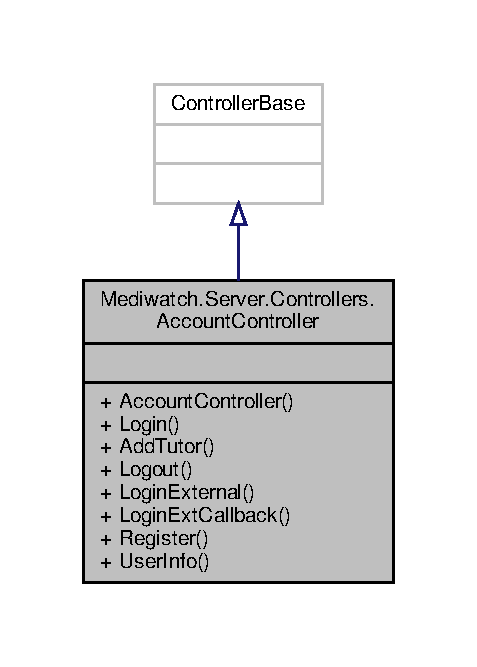
\includegraphics[width=229pt]{class_mediwatch_1_1_server_1_1_controllers_1_1_account_controller__inherit__graph}
\end{center}
\end{figure}


Graphe de collaboration de Mediwatch.\+Server.\+Controllers.\+Account\+Controller\+:\nopagebreak
\begin{figure}[H]
\begin{center}
\leavevmode
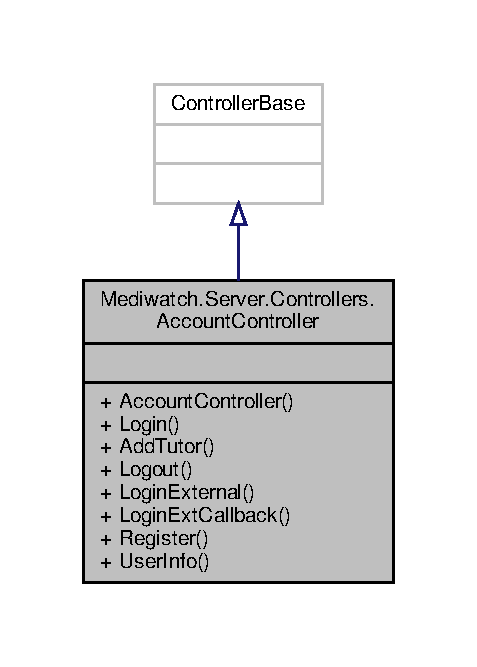
\includegraphics[width=229pt]{class_mediwatch_1_1_server_1_1_controllers_1_1_account_controller__coll__graph}
\end{center}
\end{figure}
\subsection*{Fonctions membres publiques}
\begin{DoxyCompactItemize}
\item 
\mbox{\Hypertarget{class_mediwatch_1_1_server_1_1_controllers_1_1_account_controller_ad0ec04a26c733fb1f349f7486ea820b4}\label{class_mediwatch_1_1_server_1_1_controllers_1_1_account_controller_ad0ec04a26c733fb1f349f7486ea820b4}} 
{\bfseries Account\+Controller} (Sign\+In\+Manager$<$ Identity\+User $>$ sign\+In\+Manager, User\+Manager$<$ Identity\+User $>$ user\+Manager, Role\+Manager$<$ Identity\+Role $>$ role\+Manager)
\item 
\mbox{\Hypertarget{class_mediwatch_1_1_server_1_1_controllers_1_1_account_controller_a0eca1869d875e9cdfbc6e9bc4540ae41}\label{class_mediwatch_1_1_server_1_1_controllers_1_1_account_controller_a0eca1869d875e9cdfbc6e9bc4540ae41}} 
async Task$<$ I\+Action\+Result $>$ {\bfseries Login} (Login\+Form login)
\item 
\mbox{\Hypertarget{class_mediwatch_1_1_server_1_1_controllers_1_1_account_controller_ab2521eccf3ab6c752eb5e414f6463528}\label{class_mediwatch_1_1_server_1_1_controllers_1_1_account_controller_ab2521eccf3ab6c752eb5e414f6463528}} 
async Task$<$ I\+Action\+Result $>$ {\bfseries Add\+Tutor} (string username)
\item 
\mbox{\Hypertarget{class_mediwatch_1_1_server_1_1_controllers_1_1_account_controller_a177b908ddf5a0c4ec5e3269e4cbcb252}\label{class_mediwatch_1_1_server_1_1_controllers_1_1_account_controller_a177b908ddf5a0c4ec5e3269e4cbcb252}} 
async Task$<$ I\+Action\+Result $>$ {\bfseries Logout} ()
\item 
\mbox{\Hypertarget{class_mediwatch_1_1_server_1_1_controllers_1_1_account_controller_a7f1a46f59d4b8fff4e948992fcf9f605}\label{class_mediwatch_1_1_server_1_1_controllers_1_1_account_controller_a7f1a46f59d4b8fff4e948992fcf9f605}} 
I\+Action\+Result {\bfseries Login\+External} (string hey)
\item 
\mbox{\Hypertarget{class_mediwatch_1_1_server_1_1_controllers_1_1_account_controller_ab3cb65a34f1dd5de150ebf5b956ff414}\label{class_mediwatch_1_1_server_1_1_controllers_1_1_account_controller_ab3cb65a34f1dd5de150ebf5b956ff414}} 
async Task$<$ I\+Action\+Result $>$ {\bfseries Login\+Ext\+Callback} (string return\+Url, string remote\+Error=null)
\item 
\mbox{\Hypertarget{class_mediwatch_1_1_server_1_1_controllers_1_1_account_controller_a0a0cf410c96bdacc714cb77c1d52861d}\label{class_mediwatch_1_1_server_1_1_controllers_1_1_account_controller_a0a0cf410c96bdacc714cb77c1d52861d}} 
async Task$<$ I\+Action\+Result $>$ {\bfseries Register} (Register\+Form register)
\item 
\mbox{\Hypertarget{class_mediwatch_1_1_server_1_1_controllers_1_1_account_controller_a35118ac6cb00d088863119bf4cbdc30f}\label{class_mediwatch_1_1_server_1_1_controllers_1_1_account_controller_a35118ac6cb00d088863119bf4cbdc30f}} 
User\+Information {\bfseries User\+Info} ()
\end{DoxyCompactItemize}


La documentation de cette classe a été générée à partir du fichier suivant \+:\begin{DoxyCompactItemize}
\item 
Server/\+Controllers/Account\+Controller.\+cs\end{DoxyCompactItemize}

\hypertarget{class_mediwatch_1_1_server_1_1_controllers_1_1_applicant_session_controller}{}\section{Référence de la classe Mediwatch.\+Server.\+Controllers.\+Applicant\+Session\+Controller}
\label{class_mediwatch_1_1_server_1_1_controllers_1_1_applicant_session_controller}\index{Mediwatch.\+Server.\+Controllers.\+Applicant\+Session\+Controller@{Mediwatch.\+Server.\+Controllers.\+Applicant\+Session\+Controller}}


Graphe d\textquotesingle{}héritage de Mediwatch.\+Server.\+Controllers.\+Applicant\+Session\+Controller\+:\nopagebreak
\begin{figure}[H]
\begin{center}
\leavevmode
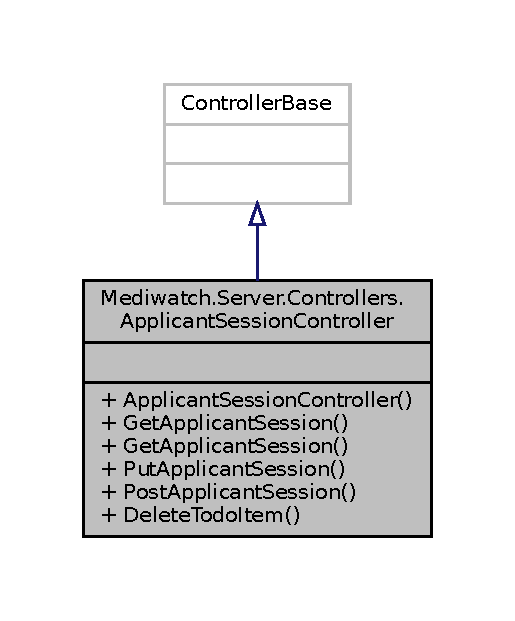
\includegraphics[width=229pt]{class_mediwatch_1_1_server_1_1_controllers_1_1_applicant_session_controller__inherit__graph}
\end{center}
\end{figure}


Graphe de collaboration de Mediwatch.\+Server.\+Controllers.\+Applicant\+Session\+Controller\+:\nopagebreak
\begin{figure}[H]
\begin{center}
\leavevmode
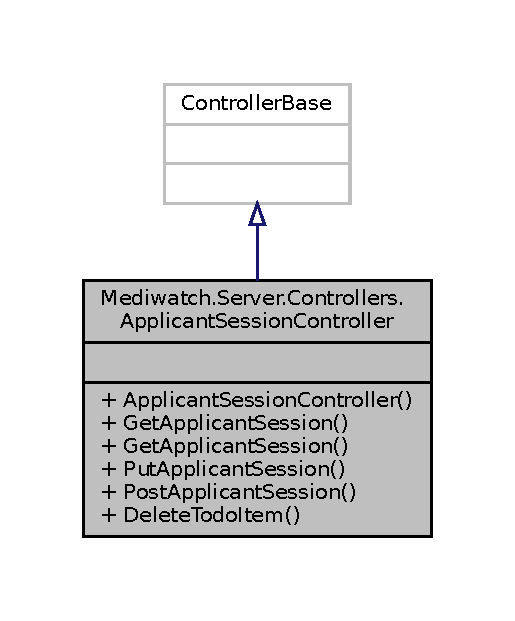
\includegraphics[width=229pt]{class_mediwatch_1_1_server_1_1_controllers_1_1_applicant_session_controller__coll__graph}
\end{center}
\end{figure}
\subsection*{Fonctions membres publiques}
\begin{DoxyCompactItemize}
\item 
\mbox{\Hypertarget{class_mediwatch_1_1_server_1_1_controllers_1_1_applicant_session_controller_a25bd4d18e93861e4d99e672b127db48b}\label{class_mediwatch_1_1_server_1_1_controllers_1_1_applicant_session_controller_a25bd4d18e93861e4d99e672b127db48b}} 
{\bfseries Applicant\+Session\+Controller} (\hyperlink{class_server_1_1_db_context_mediwatch}{Db\+Context\+Mediwatch} context)
\item 
\mbox{\Hypertarget{class_mediwatch_1_1_server_1_1_controllers_1_1_applicant_session_controller_adf8d12f5dcaaa4395522c8febae1e735}\label{class_mediwatch_1_1_server_1_1_controllers_1_1_applicant_session_controller_adf8d12f5dcaaa4395522c8febae1e735}} 
async Task$<$ Action\+Result$<$ I\+Enumerable$<$ applicant\+\_\+session $>$ $>$ $>$ {\bfseries Get\+Applicant\+Session} ()
\item 
\mbox{\Hypertarget{class_mediwatch_1_1_server_1_1_controllers_1_1_applicant_session_controller_ada65188cced0326a54f824a251869f02}\label{class_mediwatch_1_1_server_1_1_controllers_1_1_applicant_session_controller_ada65188cced0326a54f824a251869f02}} 
async Task$<$ Action\+Result$<$ applicant\+\_\+session $>$ $>$ {\bfseries Get\+Applicant\+Session} (int id)
\item 
\mbox{\Hypertarget{class_mediwatch_1_1_server_1_1_controllers_1_1_applicant_session_controller_a9b9428a2f0209f15ef65b1262e220234}\label{class_mediwatch_1_1_server_1_1_controllers_1_1_applicant_session_controller_a9b9428a2f0209f15ef65b1262e220234}} 
async Task$<$ Action\+Result$<$ applicant\+\_\+session $>$ $>$ {\bfseries Put\+Applicant\+Session} (int id, applicant\+\_\+session applicant\+Session\+Input)
\item 
\mbox{\Hypertarget{class_mediwatch_1_1_server_1_1_controllers_1_1_applicant_session_controller_a58d68c490175d8d0a13aa0104a36aed8}\label{class_mediwatch_1_1_server_1_1_controllers_1_1_applicant_session_controller_a58d68c490175d8d0a13aa0104a36aed8}} 
async Task$<$ Action\+Result$<$ applicant\+\_\+session $>$ $>$ {\bfseries Post\+Applicant\+Session} (applicant\+\_\+session applicant\+Session\+Body)
\item 
\mbox{\Hypertarget{class_mediwatch_1_1_server_1_1_controllers_1_1_applicant_session_controller_af3f0c4921fadd1483d25e39df7d5a857}\label{class_mediwatch_1_1_server_1_1_controllers_1_1_applicant_session_controller_af3f0c4921fadd1483d25e39df7d5a857}} 
async Task$<$ Action\+Result$<$ applicant\+\_\+session $>$ $>$ {\bfseries Delete\+Todo\+Item} (int id)
\end{DoxyCompactItemize}


La documentation de cette classe a été générée à partir du fichier suivant \+:\begin{DoxyCompactItemize}
\item 
Server/\+Controllers/Applicant\+Session\+Controller.\+cs\end{DoxyCompactItemize}

\hypertarget{class_mediwatch_1_1_server_1_1_controllers_1_1_compagny_controller}{}\doxysection{Référence de la classe Mediwatch.\+Server.\+Controllers.\+Compagny\+Controller}
\label{class_mediwatch_1_1_server_1_1_controllers_1_1_compagny_controller}\index{Mediwatch.Server.Controllers.CompagnyController@{Mediwatch.Server.Controllers.CompagnyController}}


Graphe d\textquotesingle{}héritage de Mediwatch.\+Server.\+Controllers.\+Compagny\+Controller\+:
\nopagebreak
\begin{figure}[H]
\begin{center}
\leavevmode
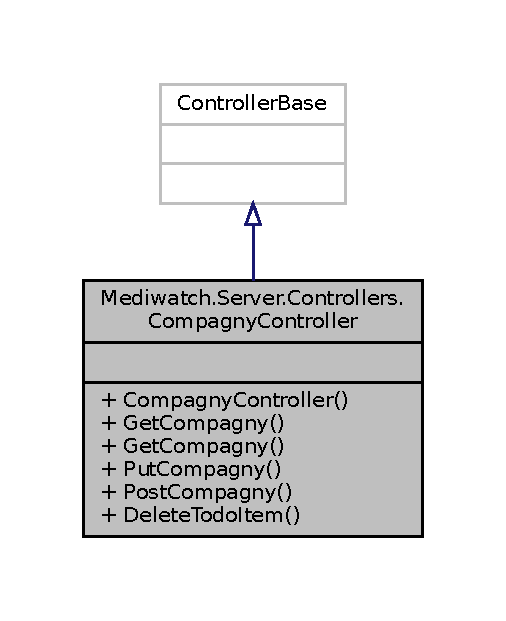
\includegraphics[width=243pt]{class_mediwatch_1_1_server_1_1_controllers_1_1_compagny_controller__inherit__graph}
\end{center}
\end{figure}


Graphe de collaboration de Mediwatch.\+Server.\+Controllers.\+Compagny\+Controller\+:
\nopagebreak
\begin{figure}[H]
\begin{center}
\leavevmode
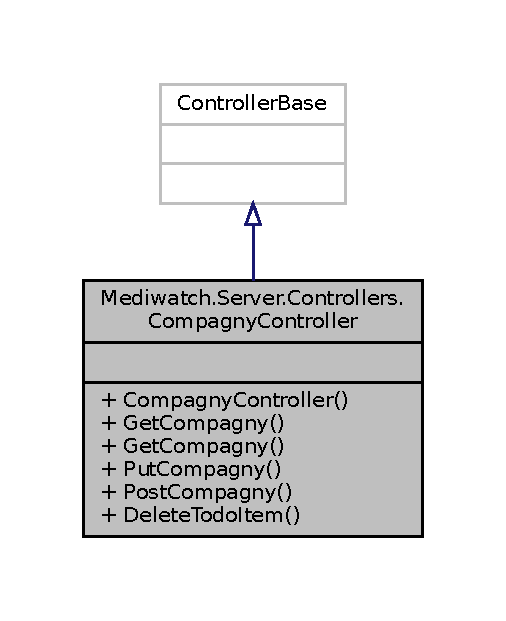
\includegraphics[width=243pt]{class_mediwatch_1_1_server_1_1_controllers_1_1_compagny_controller__coll__graph}
\end{center}
\end{figure}
\doxysubsection*{Fonctions membres publiques}
\begin{DoxyCompactItemize}
\item 
\mbox{\Hypertarget{class_mediwatch_1_1_server_1_1_controllers_1_1_compagny_controller_ab4a8837fdb737884b3248ee77f734ad0}\label{class_mediwatch_1_1_server_1_1_controllers_1_1_compagny_controller_ab4a8837fdb737884b3248ee77f734ad0}} 
{\bfseries Compagny\+Controller} (\mbox{\hyperlink{class_server_1_1_db_context_mediwatch}{Db\+Context\+Mediwatch}} context)
\item 
async Task$<$ Action\+Result$<$ I\+Enumerable$<$ compagny $>$ $>$ $>$ \mbox{\hyperlink{class_mediwatch_1_1_server_1_1_controllers_1_1_compagny_controller_a7bc69ceda49f9017a2d6ddfdbffe4758}{Get\+Compagny}} ()
\item 
async Task$<$ Action\+Result$<$ compagny $>$ $>$ \mbox{\hyperlink{class_mediwatch_1_1_server_1_1_controllers_1_1_compagny_controller_a6608c7128f9e7b31b04885ef1d7e004d}{Get\+Compagny}} (int id)
\item 
async Task$<$ Action\+Result$<$ compagny $>$ $>$ \mbox{\hyperlink{class_mediwatch_1_1_server_1_1_controllers_1_1_compagny_controller_a6d092dd8d9edcd60e4a38e1d90af3e40}{Put\+Compagny}} (int id, compagny compagny\+Input)
\item 
async Task$<$ Action\+Result$<$ compagny $>$ $>$ \mbox{\hyperlink{class_mediwatch_1_1_server_1_1_controllers_1_1_compagny_controller_ad144f627b336f3e43ba994fbdd9c9419}{Post\+Compagny}} (compagny compagny\+Body)
\item 
async Task$<$ Action\+Result$<$ compagny $>$ $>$ \mbox{\hyperlink{class_mediwatch_1_1_server_1_1_controllers_1_1_compagny_controller_a5c33b6687ecca9c5b060f029ce809e7d}{Delete\+Todo\+Item}} (int id)
\end{DoxyCompactItemize}


\doxysubsection{Documentation des fonctions membres}
\mbox{\Hypertarget{class_mediwatch_1_1_server_1_1_controllers_1_1_compagny_controller_a5c33b6687ecca9c5b060f029ce809e7d}\label{class_mediwatch_1_1_server_1_1_controllers_1_1_compagny_controller_a5c33b6687ecca9c5b060f029ce809e7d}} 
\index{Mediwatch.Server.Controllers.CompagnyController@{Mediwatch.Server.Controllers.CompagnyController}!DeleteTodoItem@{DeleteTodoItem}}
\index{DeleteTodoItem@{DeleteTodoItem}!Mediwatch.Server.Controllers.CompagnyController@{Mediwatch.Server.Controllers.CompagnyController}}
\doxysubsubsection{\texorpdfstring{DeleteTodoItem()}{DeleteTodoItem()}}
{\footnotesize\ttfamily async Task$<$Action\+Result$<$compagny$>$ $>$ Mediwatch.\+Server.\+Controllers.\+Compagny\+Controller.\+Delete\+Todo\+Item (\begin{DoxyParamCaption}\item[{int}]{id }\end{DoxyParamCaption})\hspace{0.3cm}{\ttfamily [inline]}}

Delete the company ID 

\begin{DoxyReturn}{Renvoie}

\end{DoxyReturn}
\mbox{\Hypertarget{class_mediwatch_1_1_server_1_1_controllers_1_1_compagny_controller_a7bc69ceda49f9017a2d6ddfdbffe4758}\label{class_mediwatch_1_1_server_1_1_controllers_1_1_compagny_controller_a7bc69ceda49f9017a2d6ddfdbffe4758}} 
\index{Mediwatch.Server.Controllers.CompagnyController@{Mediwatch.Server.Controllers.CompagnyController}!GetCompagny@{GetCompagny}}
\index{GetCompagny@{GetCompagny}!Mediwatch.Server.Controllers.CompagnyController@{Mediwatch.Server.Controllers.CompagnyController}}
\doxysubsubsection{\texorpdfstring{GetCompagny()}{GetCompagny()}\hspace{0.1cm}{\footnotesize\ttfamily [1/2]}}
{\footnotesize\ttfamily async Task$<$Action\+Result$<$I\+Enumerable$<$compagny$>$ $>$ $>$ Mediwatch.\+Server.\+Controllers.\+Compagny\+Controller.\+Get\+Compagny (\begin{DoxyParamCaption}{ }\end{DoxyParamCaption})\hspace{0.3cm}{\ttfamily [inline]}}

Get all compagny 

\begin{DoxyReturn}{Renvoie}
Json raw list of compgny
\end{DoxyReturn}
\mbox{\Hypertarget{class_mediwatch_1_1_server_1_1_controllers_1_1_compagny_controller_a6608c7128f9e7b31b04885ef1d7e004d}\label{class_mediwatch_1_1_server_1_1_controllers_1_1_compagny_controller_a6608c7128f9e7b31b04885ef1d7e004d}} 
\index{Mediwatch.Server.Controllers.CompagnyController@{Mediwatch.Server.Controllers.CompagnyController}!GetCompagny@{GetCompagny}}
\index{GetCompagny@{GetCompagny}!Mediwatch.Server.Controllers.CompagnyController@{Mediwatch.Server.Controllers.CompagnyController}}
\doxysubsubsection{\texorpdfstring{GetCompagny()}{GetCompagny()}\hspace{0.1cm}{\footnotesize\ttfamily [2/2]}}
{\footnotesize\ttfamily async Task$<$Action\+Result$<$compagny$>$ $>$ Mediwatch.\+Server.\+Controllers.\+Compagny\+Controller.\+Get\+Compagny (\begin{DoxyParamCaption}\item[{int}]{id }\end{DoxyParamCaption})\hspace{0.3cm}{\ttfamily [inline]}}

Get a compagny by its id 

\begin{DoxyReturn}{Renvoie}
Return the company data
\end{DoxyReturn}
\mbox{\Hypertarget{class_mediwatch_1_1_server_1_1_controllers_1_1_compagny_controller_ad144f627b336f3e43ba994fbdd9c9419}\label{class_mediwatch_1_1_server_1_1_controllers_1_1_compagny_controller_ad144f627b336f3e43ba994fbdd9c9419}} 
\index{Mediwatch.Server.Controllers.CompagnyController@{Mediwatch.Server.Controllers.CompagnyController}!PostCompagny@{PostCompagny}}
\index{PostCompagny@{PostCompagny}!Mediwatch.Server.Controllers.CompagnyController@{Mediwatch.Server.Controllers.CompagnyController}}
\doxysubsubsection{\texorpdfstring{PostCompagny()}{PostCompagny()}}
{\footnotesize\ttfamily async Task$<$Action\+Result$<$compagny$>$ $>$ Mediwatch.\+Server.\+Controllers.\+Compagny\+Controller.\+Post\+Compagny (\begin{DoxyParamCaption}\item[{compagny}]{compagny\+Body }\end{DoxyParamCaption})\hspace{0.3cm}{\ttfamily [inline]}}

Create a new compagny \mbox{\Hypertarget{class_mediwatch_1_1_server_1_1_controllers_1_1_compagny_controller_a6d092dd8d9edcd60e4a38e1d90af3e40}\label{class_mediwatch_1_1_server_1_1_controllers_1_1_compagny_controller_a6d092dd8d9edcd60e4a38e1d90af3e40}} 
\index{Mediwatch.Server.Controllers.CompagnyController@{Mediwatch.Server.Controllers.CompagnyController}!PutCompagny@{PutCompagny}}
\index{PutCompagny@{PutCompagny}!Mediwatch.Server.Controllers.CompagnyController@{Mediwatch.Server.Controllers.CompagnyController}}
\doxysubsubsection{\texorpdfstring{PutCompagny()}{PutCompagny()}}
{\footnotesize\ttfamily async Task$<$Action\+Result$<$compagny$>$ $>$ Mediwatch.\+Server.\+Controllers.\+Compagny\+Controller.\+Put\+Compagny (\begin{DoxyParamCaption}\item[{int}]{id,  }\item[{compagny}]{compagny\+Input }\end{DoxyParamCaption})\hspace{0.3cm}{\ttfamily [inline]}}

Edit the compagny information specified by its id 

~\newline


La documentation de cette classe a été générée à partir du fichier suivant \+:\begin{DoxyCompactItemize}
\item 
Server/\+Controllers/Compagny\+Controller.\+cs\end{DoxyCompactItemize}

\hypertarget{class_server_1_1_db_context_mediwatch}{}\doxysection{Référence de la classe Server.\+Db\+Context\+Mediwatch}
\label{class_server_1_1_db_context_mediwatch}\index{Server.DbContextMediwatch@{Server.DbContextMediwatch}}


Graphe d\textquotesingle{}héritage de Server.\+Db\+Context\+Mediwatch\+:
\nopagebreak
\begin{figure}[H]
\begin{center}
\leavevmode
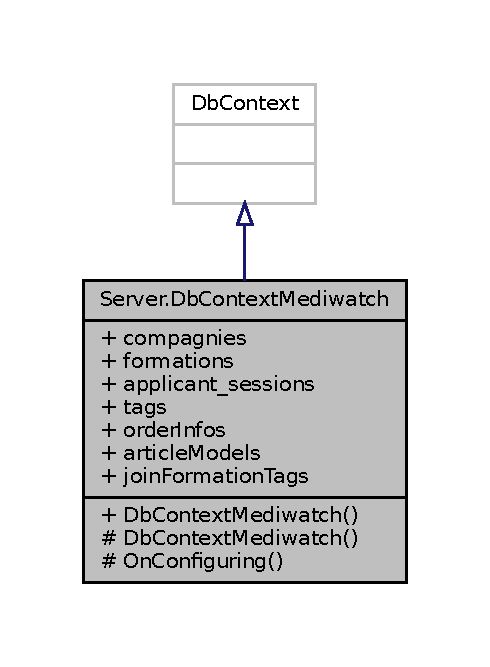
\includegraphics[width=235pt]{class_server_1_1_db_context_mediwatch__inherit__graph}
\end{center}
\end{figure}


Graphe de collaboration de Server.\+Db\+Context\+Mediwatch\+:
\nopagebreak
\begin{figure}[H]
\begin{center}
\leavevmode
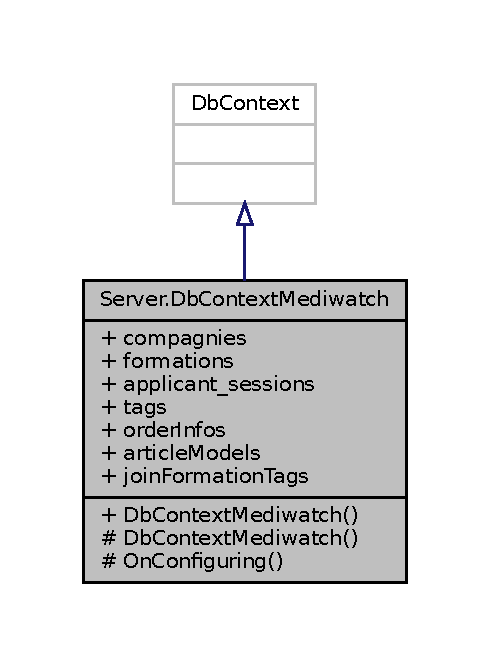
\includegraphics[width=235pt]{class_server_1_1_db_context_mediwatch__coll__graph}
\end{center}
\end{figure}
\doxysubsection*{Fonctions membres publiques}
\begin{DoxyCompactItemize}
\item 
\mbox{\Hypertarget{class_server_1_1_db_context_mediwatch_a94fde86883fe0a2d1ce0b4c58f06727f}\label{class_server_1_1_db_context_mediwatch_a94fde86883fe0a2d1ce0b4c58f06727f}} 
{\bfseries Db\+Context\+Mediwatch} (Db\+Context\+Options$<$ \mbox{\hyperlink{class_server_1_1_db_context_mediwatch}{Db\+Context\+Mediwatch}} $>$ options)
\end{DoxyCompactItemize}
\doxysubsection*{Fonctions membres protégées}
\begin{DoxyCompactItemize}
\item 
\mbox{\Hypertarget{class_server_1_1_db_context_mediwatch_a72073ff88f3990c4792f85688f55f073}\label{class_server_1_1_db_context_mediwatch_a72073ff88f3990c4792f85688f55f073}} 
override void {\bfseries On\+Configuring} (Db\+Context\+Options\+Builder options)
\end{DoxyCompactItemize}
\doxysubsection*{Propriétés}
\begin{DoxyCompactItemize}
\item 
\mbox{\Hypertarget{class_server_1_1_db_context_mediwatch_a068d9222b8448c069c2d181a9f577d0c}\label{class_server_1_1_db_context_mediwatch_a068d9222b8448c069c2d181a9f577d0c}} 
Db\+Set$<$ compagny $>$ {\bfseries compagnies}\hspace{0.3cm}{\ttfamily  \mbox{[}get, set\mbox{]}}
\item 
\mbox{\Hypertarget{class_server_1_1_db_context_mediwatch_a6597dab2848cd5aa87774af4bf6eb4e4}\label{class_server_1_1_db_context_mediwatch_a6597dab2848cd5aa87774af4bf6eb4e4}} 
Db\+Set$<$ formation $>$ {\bfseries formations}\hspace{0.3cm}{\ttfamily  \mbox{[}get, set\mbox{]}}
\item 
\mbox{\Hypertarget{class_server_1_1_db_context_mediwatch_aea8aaf9d1c1f27f64a2a488f41c531b2}\label{class_server_1_1_db_context_mediwatch_aea8aaf9d1c1f27f64a2a488f41c531b2}} 
Db\+Set$<$ applicant\+\_\+session $>$ {\bfseries applicant\+\_\+sessions}\hspace{0.3cm}{\ttfamily  \mbox{[}get, set\mbox{]}}
\item 
\mbox{\Hypertarget{class_server_1_1_db_context_mediwatch_a0bcaba8827c3d82857deb35923f6dcef}\label{class_server_1_1_db_context_mediwatch_a0bcaba8827c3d82857deb35923f6dcef}} 
Db\+Set$<$ tag $>$ {\bfseries tags}\hspace{0.3cm}{\ttfamily  \mbox{[}get, set\mbox{]}}
\item 
\mbox{\Hypertarget{class_server_1_1_db_context_mediwatch_a852541740bc368d71f6816d4e4c3be86}\label{class_server_1_1_db_context_mediwatch_a852541740bc368d71f6816d4e4c3be86}} 
Db\+Set$<$ order\+Info $>$ {\bfseries order\+Infos}\hspace{0.3cm}{\ttfamily  \mbox{[}get, set\mbox{]}}
\item 
\mbox{\Hypertarget{class_server_1_1_db_context_mediwatch_a298accc740bb1638718fe4664b41e800}\label{class_server_1_1_db_context_mediwatch_a298accc740bb1638718fe4664b41e800}} 
Db\+Set$<$ Blazing\+Article\+Model $>$ {\bfseries article\+Models}\hspace{0.3cm}{\ttfamily  \mbox{[}get, set\mbox{]}}
\end{DoxyCompactItemize}


La documentation de cette classe a été générée à partir du fichier suivant \+:\begin{DoxyCompactItemize}
\item 
Server/Db\+Context\+Mediwatch.\+cs\end{DoxyCompactItemize}

\hypertarget{class_mediwatch_1_1_server_1_1_migrations_1_1_db_context_mediwatch_migrations_1_1_db_context_mediwatch_model_snapshot}{}\doxysection{Référence de la classe Mediwatch.\+Server.\+Migrations.\+Db\+Context\+Mediwatch\+Migrations.\+Db\+Context\+Mediwatch\+Model\+Snapshot}
\label{class_mediwatch_1_1_server_1_1_migrations_1_1_db_context_mediwatch_migrations_1_1_db_context_mediwatch_model_snapshot}\index{Mediwatch.Server.Migrations.DbContextMediwatchMigrations.DbContextMediwatchModelSnapshot@{Mediwatch.Server.Migrations.DbContextMediwatchMigrations.DbContextMediwatchModelSnapshot}}


Graphe d\textquotesingle{}héritage de Mediwatch.\+Server.\+Migrations.\+Db\+Context\+Mediwatch\+Migrations.\+Db\+Context\+Mediwatch\+Model\+Snapshot\+:
\nopagebreak
\begin{figure}[H]
\begin{center}
\leavevmode
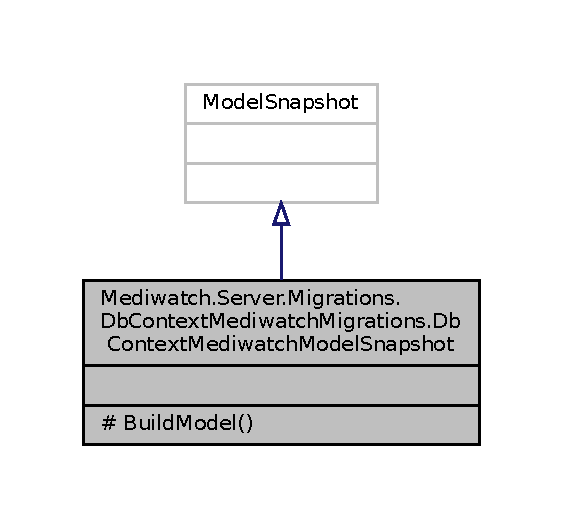
\includegraphics[width=270pt]{class_mediwatch_1_1_server_1_1_migrations_1_1_db_context_mediwatch_migrations_1_1_db_context_mede4265d04ea6c9106ce2ecf4620b99a3e}
\end{center}
\end{figure}


Graphe de collaboration de Mediwatch.\+Server.\+Migrations.\+Db\+Context\+Mediwatch\+Migrations.\+Db\+Context\+Mediwatch\+Model\+Snapshot\+:
\nopagebreak
\begin{figure}[H]
\begin{center}
\leavevmode
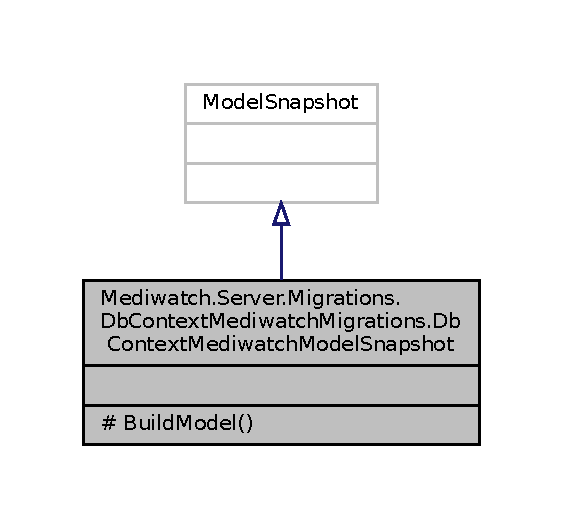
\includegraphics[width=270pt]{class_mediwatch_1_1_server_1_1_migrations_1_1_db_context_mediwatch_migrations_1_1_db_context_med877236defc748ac970f0d300226712b8}
\end{center}
\end{figure}
\doxysubsection*{Fonctions membres protégées}
\begin{DoxyCompactItemize}
\item 
\mbox{\Hypertarget{class_mediwatch_1_1_server_1_1_migrations_1_1_db_context_mediwatch_migrations_1_1_db_context_mediwatch_model_snapshot_a8cd3af8a526962ffea2f87f15691a207}\label{class_mediwatch_1_1_server_1_1_migrations_1_1_db_context_mediwatch_migrations_1_1_db_context_mediwatch_model_snapshot_a8cd3af8a526962ffea2f87f15691a207}} 
override void {\bfseries Build\+Model} (Model\+Builder model\+Builder)
\end{DoxyCompactItemize}


La documentation de cette classe a été générée à partir du fichier suivant \+:\begin{DoxyCompactItemize}
\item 
Server/\+Migrations/\+Db\+Context\+Mediwatch\+Migrations/Db\+Context\+Mediwatch\+Model\+Snapshot.\+cs\end{DoxyCompactItemize}

\hypertarget{class_mediwatch_1_1_server_1_1_pages_1_1_error_model}{}\doxysection{Référence de la classe Mediwatch.\+Server.\+Pages.\+Error\+Model}
\label{class_mediwatch_1_1_server_1_1_pages_1_1_error_model}\index{Mediwatch.Server.Pages.ErrorModel@{Mediwatch.Server.Pages.ErrorModel}}


Graphe d\textquotesingle{}héritage de Mediwatch.\+Server.\+Pages.\+Error\+Model\+:\nopagebreak
\begin{figure}[H]
\begin{center}
\leavevmode
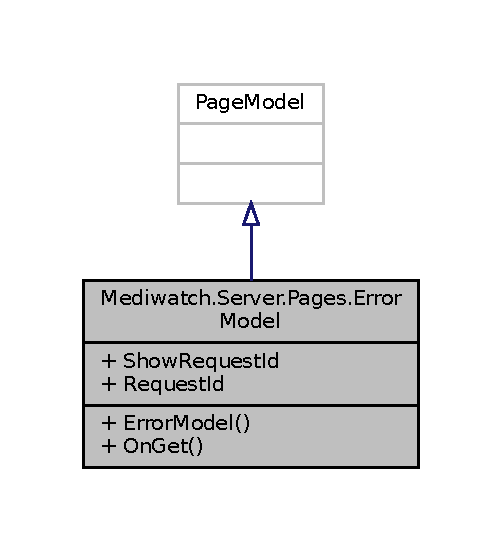
\includegraphics[width=241pt]{class_mediwatch_1_1_server_1_1_pages_1_1_error_model__inherit__graph}
\end{center}
\end{figure}


Graphe de collaboration de Mediwatch.\+Server.\+Pages.\+Error\+Model\+:\nopagebreak
\begin{figure}[H]
\begin{center}
\leavevmode
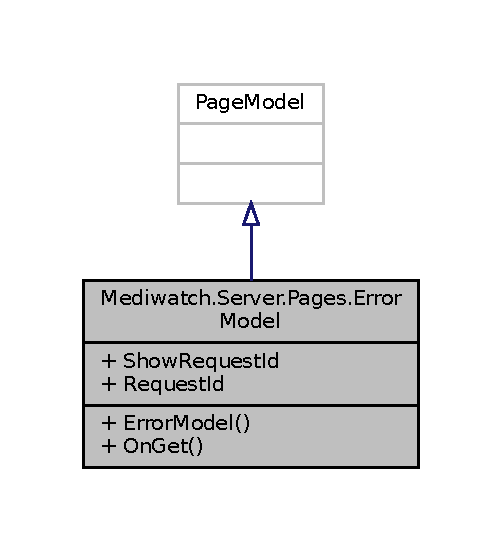
\includegraphics[width=241pt]{class_mediwatch_1_1_server_1_1_pages_1_1_error_model__coll__graph}
\end{center}
\end{figure}
\doxysubsection*{Fonctions membres publiques}
\begin{DoxyCompactItemize}
\item 
\mbox{\Hypertarget{class_mediwatch_1_1_server_1_1_pages_1_1_error_model_a6071f8072c63f30c32dac09a811f9ab3}\label{class_mediwatch_1_1_server_1_1_pages_1_1_error_model_a6071f8072c63f30c32dac09a811f9ab3}} 
{\bfseries Error\+Model} (I\+Logger$<$ \mbox{\hyperlink{class_mediwatch_1_1_server_1_1_pages_1_1_error_model}{Error\+Model}} $>$ logger)
\item 
\mbox{\Hypertarget{class_mediwatch_1_1_server_1_1_pages_1_1_error_model_afff141d7facfcb25a4a05e433cb18369}\label{class_mediwatch_1_1_server_1_1_pages_1_1_error_model_afff141d7facfcb25a4a05e433cb18369}} 
void {\bfseries On\+Get} ()
\end{DoxyCompactItemize}
\doxysubsection*{Attributs publics}
\begin{DoxyCompactItemize}
\item 
\mbox{\Hypertarget{class_mediwatch_1_1_server_1_1_pages_1_1_error_model_a63bd289fd620d1418adcd60cc4ff7f53}\label{class_mediwatch_1_1_server_1_1_pages_1_1_error_model_a63bd289fd620d1418adcd60cc4ff7f53}} 
bool {\bfseries Show\+Request\+Id} =$>$ !string.\+Is\+Null\+Or\+Empty(Request\+Id)
\end{DoxyCompactItemize}
\doxysubsection*{Propriétés}
\begin{DoxyCompactItemize}
\item 
\mbox{\Hypertarget{class_mediwatch_1_1_server_1_1_pages_1_1_error_model_a6b1ab7a6328fa0b58ac9b76c0d8bfbef}\label{class_mediwatch_1_1_server_1_1_pages_1_1_error_model_a6b1ab7a6328fa0b58ac9b76c0d8bfbef}} 
string {\bfseries Request\+Id}\hspace{0.3cm}{\ttfamily  \mbox{[}get, set\mbox{]}}
\end{DoxyCompactItemize}


La documentation de cette classe a été générée à partir du fichier suivant \+:\begin{DoxyCompactItemize}
\item 
Server/\+Pages/Error.\+cshtml.\+cs\end{DoxyCompactItemize}

\hypertarget{class_mediwatch_1_1_server_1_1_controllers_1_1_formation_controller}{}\doxysection{Référence de la classe Mediwatch.\+Server.\+Controllers.\+Formation\+Controller}
\label{class_mediwatch_1_1_server_1_1_controllers_1_1_formation_controller}\index{Mediwatch.Server.Controllers.FormationController@{Mediwatch.Server.Controllers.FormationController}}


Graphe d\textquotesingle{}héritage de Mediwatch.\+Server.\+Controllers.\+Formation\+Controller\+:
\nopagebreak
\begin{figure}[H]
\begin{center}
\leavevmode
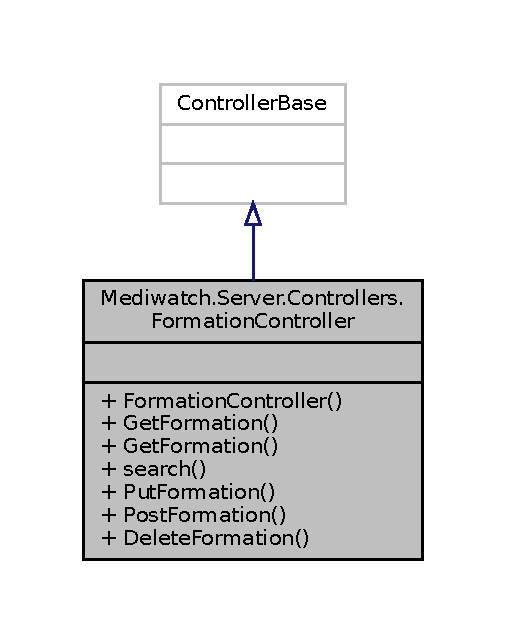
\includegraphics[width=243pt]{class_mediwatch_1_1_server_1_1_controllers_1_1_formation_controller__inherit__graph}
\end{center}
\end{figure}


Graphe de collaboration de Mediwatch.\+Server.\+Controllers.\+Formation\+Controller\+:
\nopagebreak
\begin{figure}[H]
\begin{center}
\leavevmode
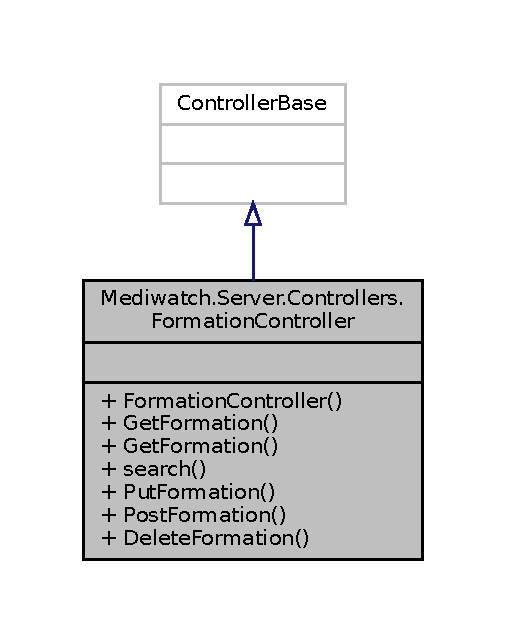
\includegraphics[width=243pt]{class_mediwatch_1_1_server_1_1_controllers_1_1_formation_controller__coll__graph}
\end{center}
\end{figure}
\doxysubsection*{Fonctions membres publiques}
\begin{DoxyCompactItemize}
\item 
\mbox{\Hypertarget{class_mediwatch_1_1_server_1_1_controllers_1_1_formation_controller_a71430327b82736d6b252d83a40833dbd}\label{class_mediwatch_1_1_server_1_1_controllers_1_1_formation_controller_a71430327b82736d6b252d83a40833dbd}} 
{\bfseries Formation\+Controller} (\mbox{\hyperlink{class_server_1_1_db_context_mediwatch}{Db\+Context\+Mediwatch}} context)
\item 
async Task$<$ Action\+Result$<$ I\+Enumerable$<$ formation $>$ $>$ $>$ \mbox{\hyperlink{class_mediwatch_1_1_server_1_1_controllers_1_1_formation_controller_ac1711d7a1c8bbd44715fc57cb945c93c}{Get\+Formation}} ()
\item 
async Task$<$ Action\+Result$<$ formation $>$ $>$ \mbox{\hyperlink{class_mediwatch_1_1_server_1_1_controllers_1_1_formation_controller_aecf887fc57ba8ee1af0ba1be7703738a}{Get\+Formation}} (int id)
\item 
async Task$<$ Action\+Result$<$ formation $>$ $>$ \mbox{\hyperlink{class_mediwatch_1_1_server_1_1_controllers_1_1_formation_controller_ac56853c9a6cf3b7cb2303d1c6bf8a037}{Put\+Formation}} (int id, formation formation\+Put)
\item 
async Task$<$ Action\+Result$<$ formation $>$ $>$ \mbox{\hyperlink{class_mediwatch_1_1_server_1_1_controllers_1_1_formation_controller_a2710e701c2d495ee6a1d343a5303bfa3}{Post\+Formation}} (formation formation\+Body)
\item 
async Task$<$ Action\+Result$<$ formation $>$ $>$ \mbox{\hyperlink{class_mediwatch_1_1_server_1_1_controllers_1_1_formation_controller_af3e300009a2f7d0d1551da387effbe09}{Delete\+Formation}} (int id)
\end{DoxyCompactItemize}


\doxysubsection{Documentation des fonctions membres}
\mbox{\Hypertarget{class_mediwatch_1_1_server_1_1_controllers_1_1_formation_controller_af3e300009a2f7d0d1551da387effbe09}\label{class_mediwatch_1_1_server_1_1_controllers_1_1_formation_controller_af3e300009a2f7d0d1551da387effbe09}} 
\index{Mediwatch.Server.Controllers.FormationController@{Mediwatch.Server.Controllers.FormationController}!DeleteFormation@{DeleteFormation}}
\index{DeleteFormation@{DeleteFormation}!Mediwatch.Server.Controllers.FormationController@{Mediwatch.Server.Controllers.FormationController}}
\doxysubsubsection{\texorpdfstring{DeleteFormation()}{DeleteFormation()}}
{\footnotesize\ttfamily async Task$<$Action\+Result$<$formation$>$ $>$ Mediwatch.\+Server.\+Controllers.\+Formation\+Controller.\+Delete\+Formation (\begin{DoxyParamCaption}\item[{int}]{id }\end{DoxyParamCaption})\hspace{0.3cm}{\ttfamily [inline]}}

Delete the formation by ID 

\begin{DoxyReturn}{Renvoie}

\end{DoxyReturn}
\mbox{\Hypertarget{class_mediwatch_1_1_server_1_1_controllers_1_1_formation_controller_ac1711d7a1c8bbd44715fc57cb945c93c}\label{class_mediwatch_1_1_server_1_1_controllers_1_1_formation_controller_ac1711d7a1c8bbd44715fc57cb945c93c}} 
\index{Mediwatch.Server.Controllers.FormationController@{Mediwatch.Server.Controllers.FormationController}!GetFormation@{GetFormation}}
\index{GetFormation@{GetFormation}!Mediwatch.Server.Controllers.FormationController@{Mediwatch.Server.Controllers.FormationController}}
\doxysubsubsection{\texorpdfstring{GetFormation()}{GetFormation()}\hspace{0.1cm}{\footnotesize\ttfamily [1/2]}}
{\footnotesize\ttfamily async Task$<$Action\+Result$<$I\+Enumerable$<$formation$>$ $>$ $>$ Mediwatch.\+Server.\+Controllers.\+Formation\+Controller.\+Get\+Formation (\begin{DoxyParamCaption}{ }\end{DoxyParamCaption})\hspace{0.3cm}{\ttfamily [inline]}}

Get all formation 

\begin{DoxyReturn}{Renvoie}
Return the list of the available formation
\end{DoxyReturn}
\mbox{\Hypertarget{class_mediwatch_1_1_server_1_1_controllers_1_1_formation_controller_aecf887fc57ba8ee1af0ba1be7703738a}\label{class_mediwatch_1_1_server_1_1_controllers_1_1_formation_controller_aecf887fc57ba8ee1af0ba1be7703738a}} 
\index{Mediwatch.Server.Controllers.FormationController@{Mediwatch.Server.Controllers.FormationController}!GetFormation@{GetFormation}}
\index{GetFormation@{GetFormation}!Mediwatch.Server.Controllers.FormationController@{Mediwatch.Server.Controllers.FormationController}}
\doxysubsubsection{\texorpdfstring{GetFormation()}{GetFormation()}\hspace{0.1cm}{\footnotesize\ttfamily [2/2]}}
{\footnotesize\ttfamily async Task$<$Action\+Result$<$formation$>$ $>$ Mediwatch.\+Server.\+Controllers.\+Formation\+Controller.\+Get\+Formation (\begin{DoxyParamCaption}\item[{int}]{id }\end{DoxyParamCaption})\hspace{0.3cm}{\ttfamily [inline]}}

Get a specific formation by is ID 

\begin{DoxyReturn}{Renvoie}
Return the formation information
\end{DoxyReturn}
\mbox{\Hypertarget{class_mediwatch_1_1_server_1_1_controllers_1_1_formation_controller_a2710e701c2d495ee6a1d343a5303bfa3}\label{class_mediwatch_1_1_server_1_1_controllers_1_1_formation_controller_a2710e701c2d495ee6a1d343a5303bfa3}} 
\index{Mediwatch.Server.Controllers.FormationController@{Mediwatch.Server.Controllers.FormationController}!PostFormation@{PostFormation}}
\index{PostFormation@{PostFormation}!Mediwatch.Server.Controllers.FormationController@{Mediwatch.Server.Controllers.FormationController}}
\doxysubsubsection{\texorpdfstring{PostFormation()}{PostFormation()}}
{\footnotesize\ttfamily async Task$<$Action\+Result$<$formation$>$ $>$ Mediwatch.\+Server.\+Controllers.\+Formation\+Controller.\+Post\+Formation (\begin{DoxyParamCaption}\item[{formation}]{formation\+Body }\end{DoxyParamCaption})\hspace{0.3cm}{\ttfamily [inline]}}

Create a new formation \mbox{\Hypertarget{class_mediwatch_1_1_server_1_1_controllers_1_1_formation_controller_ac56853c9a6cf3b7cb2303d1c6bf8a037}\label{class_mediwatch_1_1_server_1_1_controllers_1_1_formation_controller_ac56853c9a6cf3b7cb2303d1c6bf8a037}} 
\index{Mediwatch.Server.Controllers.FormationController@{Mediwatch.Server.Controllers.FormationController}!PutFormation@{PutFormation}}
\index{PutFormation@{PutFormation}!Mediwatch.Server.Controllers.FormationController@{Mediwatch.Server.Controllers.FormationController}}
\doxysubsubsection{\texorpdfstring{PutFormation()}{PutFormation()}}
{\footnotesize\ttfamily async Task$<$Action\+Result$<$formation$>$ $>$ Mediwatch.\+Server.\+Controllers.\+Formation\+Controller.\+Put\+Formation (\begin{DoxyParamCaption}\item[{int}]{id,  }\item[{formation}]{formation\+Put }\end{DoxyParamCaption})\hspace{0.3cm}{\ttfamily [inline]}}

Update the formation specific by is ID 

La documentation de cette classe a été générée à partir du fichier suivant \+:\begin{DoxyCompactItemize}
\item 
Server/\+Controllers/Formation\+Controller.\+cs\end{DoxyCompactItemize}

\hypertarget{class_mediwatch_1_1_server_1_1_areas_1_1_identity_1_1_data_1_1_identity_data_context}{}\section{Référence de la classe Mediwatch.\+Server.\+Areas.\+Identity.\+Data.\+Identity\+Data\+Context}
\label{class_mediwatch_1_1_server_1_1_areas_1_1_identity_1_1_data_1_1_identity_data_context}\index{Mediwatch.\+Server.\+Areas.\+Identity.\+Data.\+Identity\+Data\+Context@{Mediwatch.\+Server.\+Areas.\+Identity.\+Data.\+Identity\+Data\+Context}}


Graphe d\textquotesingle{}héritage de Mediwatch.\+Server.\+Areas.\+Identity.\+Data.\+Identity\+Data\+Context\+:\nopagebreak
\begin{figure}[H]
\begin{center}
\leavevmode
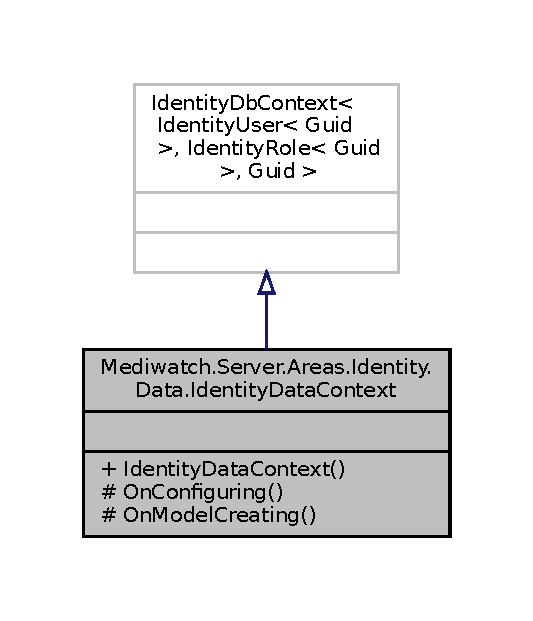
\includegraphics[width=242pt]{class_mediwatch_1_1_server_1_1_areas_1_1_identity_1_1_data_1_1_identity_data_context__inherit__graph}
\end{center}
\end{figure}


Graphe de collaboration de Mediwatch.\+Server.\+Areas.\+Identity.\+Data.\+Identity\+Data\+Context\+:\nopagebreak
\begin{figure}[H]
\begin{center}
\leavevmode
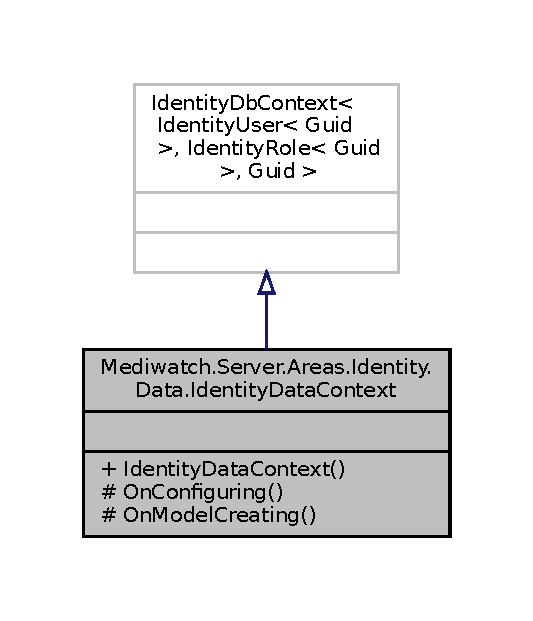
\includegraphics[width=242pt]{class_mediwatch_1_1_server_1_1_areas_1_1_identity_1_1_data_1_1_identity_data_context__coll__graph}
\end{center}
\end{figure}
\subsection*{Fonctions membres publiques}
\begin{DoxyCompactItemize}
\item 
\mbox{\Hypertarget{class_mediwatch_1_1_server_1_1_areas_1_1_identity_1_1_data_1_1_identity_data_context_ace53da6e49b7d2dff2bb67aad43cfa65}\label{class_mediwatch_1_1_server_1_1_areas_1_1_identity_1_1_data_1_1_identity_data_context_ace53da6e49b7d2dff2bb67aad43cfa65}} 
{\bfseries Identity\+Data\+Context} (Db\+Context\+Options$<$ \hyperlink{class_mediwatch_1_1_server_1_1_areas_1_1_identity_1_1_data_1_1_identity_data_context}{Identity\+Data\+Context} $>$ options)
\end{DoxyCompactItemize}
\subsection*{Fonctions membres protégées}
\begin{DoxyCompactItemize}
\item 
\mbox{\Hypertarget{class_mediwatch_1_1_server_1_1_areas_1_1_identity_1_1_data_1_1_identity_data_context_aa038bee1336ce8e66954bc5cfdc52e7a}\label{class_mediwatch_1_1_server_1_1_areas_1_1_identity_1_1_data_1_1_identity_data_context_aa038bee1336ce8e66954bc5cfdc52e7a}} 
override void {\bfseries On\+Model\+Creating} (Model\+Builder builder)
\end{DoxyCompactItemize}


La documentation de cette classe a été générée à partir du fichier suivant \+:\begin{DoxyCompactItemize}
\item 
Server/\+Areas/\+Identity/\+Data/Identity\+Data\+Context.\+cs\end{DoxyCompactItemize}

\hypertarget{class_mediwatch_1_1_server_1_1_migrations_1_1_identity_data_context_model_snapshot}{}\doxysection{Référence de la classe Mediwatch.\+Server.\+Migrations.\+Identity\+Data\+Context\+Model\+Snapshot}
\label{class_mediwatch_1_1_server_1_1_migrations_1_1_identity_data_context_model_snapshot}\index{Mediwatch.Server.Migrations.IdentityDataContextModelSnapshot@{Mediwatch.Server.Migrations.IdentityDataContextModelSnapshot}}


Graphe d\textquotesingle{}héritage de Mediwatch.\+Server.\+Migrations.\+Identity\+Data\+Context\+Model\+Snapshot\+:
% FIG 0


Graphe de collaboration de Mediwatch.\+Server.\+Migrations.\+Identity\+Data\+Context\+Model\+Snapshot\+:
% FIG 1
\doxysubsection*{Fonctions membres protégées}
\begin{DoxyCompactItemize}
\item 
override void \mbox{\hyperlink{class_mediwatch_1_1_server_1_1_migrations_1_1_identity_data_context_model_snapshot_a0d86a793fac77b235571009b08163338}{Build\+Model}} (Model\+Builder model\+Builder)
\end{DoxyCompactItemize}


\doxysubsection{Documentation des fonctions membres}
\mbox{\Hypertarget{class_mediwatch_1_1_server_1_1_migrations_1_1_identity_data_context_model_snapshot_a0d86a793fac77b235571009b08163338}\label{class_mediwatch_1_1_server_1_1_migrations_1_1_identity_data_context_model_snapshot_a0d86a793fac77b235571009b08163338}} 
\index{Mediwatch.Server.Migrations.IdentityDataContextModelSnapshot@{Mediwatch.Server.Migrations.IdentityDataContextModelSnapshot}!BuildModel@{BuildModel}}
\index{BuildModel@{BuildModel}!Mediwatch.Server.Migrations.IdentityDataContextModelSnapshot@{Mediwatch.Server.Migrations.IdentityDataContextModelSnapshot}}
\doxysubsubsection{\texorpdfstring{BuildModel()}{BuildModel()}}
{\footnotesize\ttfamily override void Mediwatch.\+Server.\+Migrations.\+Identity\+Data\+Context\+Model\+Snapshot.\+Build\+Model (\begin{DoxyParamCaption}\item[{Model\+Builder}]{model\+Builder }\end{DoxyParamCaption})\hspace{0.3cm}{\ttfamily [protected]}}



La documentation de cette classe a été générée à partir du fichier suivant \+:\begin{DoxyCompactItemize}
\item 
Server/\+Migrations/\mbox{\hyperlink{_identity_data_context_model_snapshot_8cs}{Identity\+Data\+Context\+Model\+Snapshot.\+cs}}\end{DoxyCompactItemize}

\hypertarget{class_mediwatch_1_1_server_1_1_areas_1_1_identity_1_1_identity_hosting_startup}{}\doxysection{Référence de la classe Mediwatch.\+Server.\+Areas.\+Identity.\+Identity\+Hosting\+Startup}
\label{class_mediwatch_1_1_server_1_1_areas_1_1_identity_1_1_identity_hosting_startup}\index{Mediwatch.Server.Areas.Identity.IdentityHostingStartup@{Mediwatch.Server.Areas.Identity.IdentityHostingStartup}}


Graphe d\textquotesingle{}héritage de Mediwatch.\+Server.\+Areas.\+Identity.\+Identity\+Hosting\+Startup\+:
\nopagebreak
\begin{figure}[H]
\begin{center}
\leavevmode
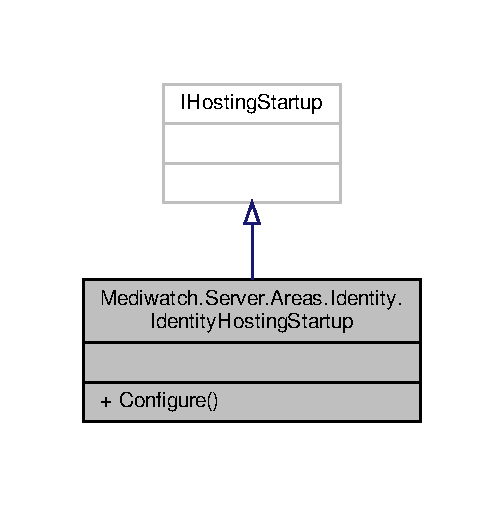
\includegraphics[width=256pt]{class_mediwatch_1_1_server_1_1_areas_1_1_identity_1_1_identity_hosting_startup__inherit__graph}
\end{center}
\end{figure}


Graphe de collaboration de Mediwatch.\+Server.\+Areas.\+Identity.\+Identity\+Hosting\+Startup\+:
\nopagebreak
\begin{figure}[H]
\begin{center}
\leavevmode
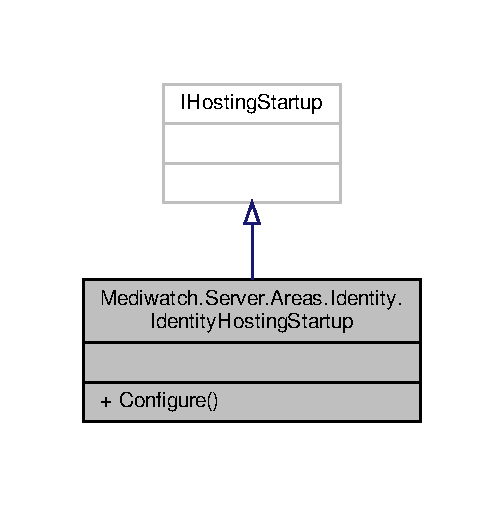
\includegraphics[width=256pt]{class_mediwatch_1_1_server_1_1_areas_1_1_identity_1_1_identity_hosting_startup__coll__graph}
\end{center}
\end{figure}
\doxysubsection*{Fonctions membres publiques}
\begin{DoxyCompactItemize}
\item 
\mbox{\Hypertarget{class_mediwatch_1_1_server_1_1_areas_1_1_identity_1_1_identity_hosting_startup_a4206ebb6e9389e9fee2397a1454f7f9b}\label{class_mediwatch_1_1_server_1_1_areas_1_1_identity_1_1_identity_hosting_startup_a4206ebb6e9389e9fee2397a1454f7f9b}} 
void {\bfseries Configure} (I\+Web\+Host\+Builder builder)
\end{DoxyCompactItemize}


La documentation de cette classe a été générée à partir du fichier suivant \+:\begin{DoxyCompactItemize}
\item 
Server/\+Areas/\+Identity/Identity\+Hosting\+Startup.\+cs\end{DoxyCompactItemize}

\hypertarget{class_mediwatch_1_1_server_1_1_migrations_1_1innitial_create}{}\doxysection{Référence de la classe Mediwatch.\+Server.\+Migrations.\+innitial\+Create}
\label{class_mediwatch_1_1_server_1_1_migrations_1_1innitial_create}\index{Mediwatch.Server.Migrations.innitialCreate@{Mediwatch.Server.Migrations.innitialCreate}}


Graphe d\textquotesingle{}héritage de Mediwatch.\+Server.\+Migrations.\+innitial\+Create\+:
\nopagebreak
\begin{figure}[H]
\begin{center}
\leavevmode
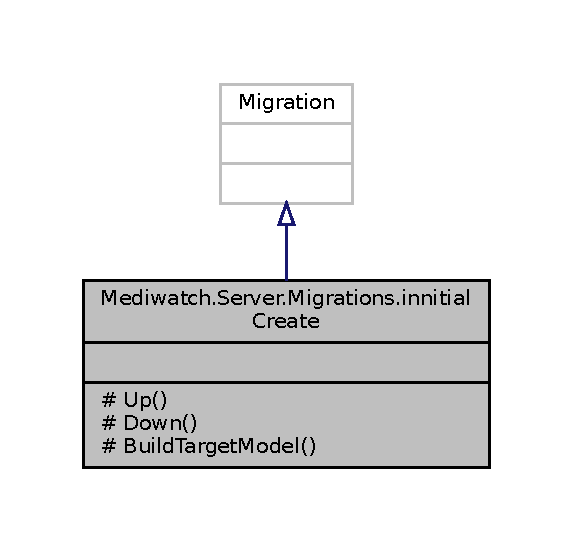
\includegraphics[width=275pt]{class_mediwatch_1_1_server_1_1_migrations_1_1innitial_create__inherit__graph}
\end{center}
\end{figure}


Graphe de collaboration de Mediwatch.\+Server.\+Migrations.\+innitial\+Create\+:
\nopagebreak
\begin{figure}[H]
\begin{center}
\leavevmode
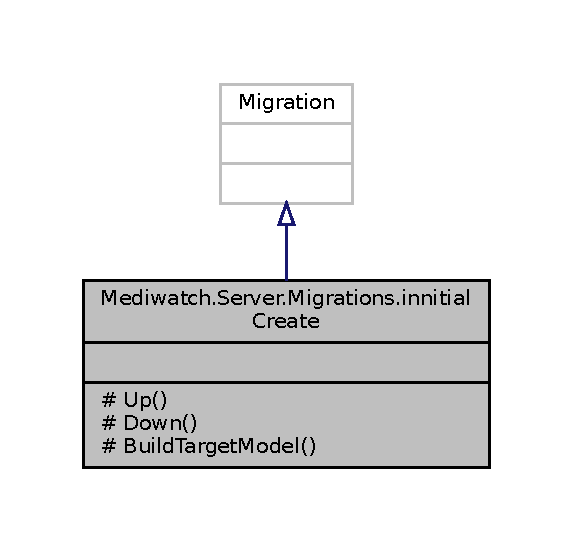
\includegraphics[width=275pt]{class_mediwatch_1_1_server_1_1_migrations_1_1innitial_create__coll__graph}
\end{center}
\end{figure}
\doxysubsection*{Fonctions membres protégées}
\begin{DoxyCompactItemize}
\item 
\mbox{\Hypertarget{class_mediwatch_1_1_server_1_1_migrations_1_1innitial_create_ae036630989af2c2f41f0b2257d35a8e0}\label{class_mediwatch_1_1_server_1_1_migrations_1_1innitial_create_ae036630989af2c2f41f0b2257d35a8e0}} 
override void {\bfseries Up} (Migration\+Builder migration\+Builder)
\item 
\mbox{\Hypertarget{class_mediwatch_1_1_server_1_1_migrations_1_1innitial_create_a8a02e197d3bd2cc0eefc6ac7814d1372}\label{class_mediwatch_1_1_server_1_1_migrations_1_1innitial_create_a8a02e197d3bd2cc0eefc6ac7814d1372}} 
override void {\bfseries Down} (Migration\+Builder migration\+Builder)
\item 
\mbox{\Hypertarget{class_mediwatch_1_1_server_1_1_migrations_1_1innitial_create_ad7cc9104c9bb7f0274826a71631b8851}\label{class_mediwatch_1_1_server_1_1_migrations_1_1innitial_create_ad7cc9104c9bb7f0274826a71631b8851}} 
override void {\bfseries Build\+Target\+Model} (Model\+Builder model\+Builder)
\end{DoxyCompactItemize}


La documentation de cette classe a été générée à partir des fichiers suivants \+:\begin{DoxyCompactItemize}
\item 
Server/\+Migrations/20210104114702\+\_\+innitial\+Create.\+cs\item 
Server/\+Migrations/20210104114702\+\_\+innitial\+Create.\+Designer.\+cs\end{DoxyCompactItemize}

\hypertarget{class_mediwatch_1_1_server_1_1_program}{}\doxysection{Référence de la classe Mediwatch.\+Server.\+Program}
\label{class_mediwatch_1_1_server_1_1_program}\index{Mediwatch.Server.Program@{Mediwatch.Server.Program}}


Graphe de collaboration de Mediwatch.\+Server.\+Program\+:
% FIG 0
\doxysubsection*{Fonctions membres publiques statiques}
\begin{DoxyCompactItemize}
\item 
static void \mbox{\hyperlink{class_mediwatch_1_1_server_1_1_program_a0b37e08654729aa1c9f3a572e5775305}{Main}} (string\mbox{[}$\,$\mbox{]} args)
\item 
static I\+Host\+Builder \mbox{\hyperlink{class_mediwatch_1_1_server_1_1_program_a5278302328dd5740238221820ef8fa07}{Create\+Host\+Builder}} (string\mbox{[}$\,$\mbox{]} args)
\end{DoxyCompactItemize}


\doxysubsection{Documentation des fonctions membres}
\mbox{\Hypertarget{class_mediwatch_1_1_server_1_1_program_a5278302328dd5740238221820ef8fa07}\label{class_mediwatch_1_1_server_1_1_program_a5278302328dd5740238221820ef8fa07}} 
\index{Mediwatch.Server.Program@{Mediwatch.Server.Program}!CreateHostBuilder@{CreateHostBuilder}}
\index{CreateHostBuilder@{CreateHostBuilder}!Mediwatch.Server.Program@{Mediwatch.Server.Program}}
\doxysubsubsection{\texorpdfstring{CreateHostBuilder()}{CreateHostBuilder()}}
{\footnotesize\ttfamily static I\+Host\+Builder Mediwatch.\+Server.\+Program.\+Create\+Host\+Builder (\begin{DoxyParamCaption}\item[{string\mbox{[}$\,$\mbox{]}}]{args }\end{DoxyParamCaption})\hspace{0.3cm}{\ttfamily [static]}}

\mbox{\Hypertarget{class_mediwatch_1_1_server_1_1_program_a0b37e08654729aa1c9f3a572e5775305}\label{class_mediwatch_1_1_server_1_1_program_a0b37e08654729aa1c9f3a572e5775305}} 
\index{Mediwatch.Server.Program@{Mediwatch.Server.Program}!Main@{Main}}
\index{Main@{Main}!Mediwatch.Server.Program@{Mediwatch.Server.Program}}
\doxysubsubsection{\texorpdfstring{Main()}{Main()}}
{\footnotesize\ttfamily static void Mediwatch.\+Server.\+Program.\+Main (\begin{DoxyParamCaption}\item[{string\mbox{[}$\,$\mbox{]}}]{args }\end{DoxyParamCaption})\hspace{0.3cm}{\ttfamily [static]}}



La documentation de cette classe a été générée à partir du fichier suivant \+:\begin{DoxyCompactItemize}
\item 
Server/\mbox{\hyperlink{_program_8cs}{Program.\+cs}}\end{DoxyCompactItemize}

\hypertarget{class_mediwatch_1_1_server_1_1_startup}{}\section{Référence de la classe Mediwatch.\+Server.\+Startup}
\label{class_mediwatch_1_1_server_1_1_startup}\index{Mediwatch.\+Server.\+Startup@{Mediwatch.\+Server.\+Startup}}


Graphe de collaboration de Mediwatch.\+Server.\+Startup\+:
\nopagebreak
\begin{figure}[H]
\begin{center}
\leavevmode
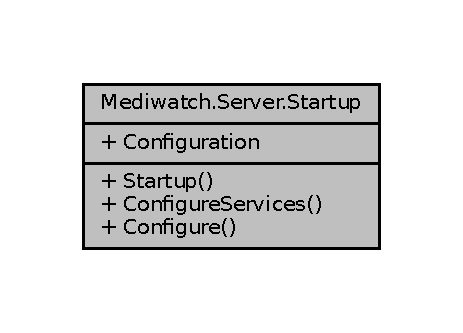
\includegraphics[width=210pt]{class_mediwatch_1_1_server_1_1_startup__coll__graph}
\end{center}
\end{figure}
\subsection*{Fonctions membres publiques}
\begin{DoxyCompactItemize}
\item 
\mbox{\Hypertarget{class_mediwatch_1_1_server_1_1_startup_a99779cbd7c184cbff98730a5f285a647}\label{class_mediwatch_1_1_server_1_1_startup_a99779cbd7c184cbff98730a5f285a647}} 
{\bfseries Startup} (I\+Configuration configuration)
\item 
\mbox{\Hypertarget{class_mediwatch_1_1_server_1_1_startup_a98b7f4b5e49a83c353687ec3c1cfa139}\label{class_mediwatch_1_1_server_1_1_startup_a98b7f4b5e49a83c353687ec3c1cfa139}} 
void {\bfseries Configure\+Services} (I\+Service\+Collection services)
\item 
\mbox{\Hypertarget{class_mediwatch_1_1_server_1_1_startup_af31b63124f79f812e79cb6f43df14a40}\label{class_mediwatch_1_1_server_1_1_startup_af31b63124f79f812e79cb6f43df14a40}} 
void {\bfseries Configure} (I\+Application\+Builder app, I\+Web\+Host\+Environment env)
\end{DoxyCompactItemize}
\subsection*{Propriétés}
\begin{DoxyCompactItemize}
\item 
\mbox{\Hypertarget{class_mediwatch_1_1_server_1_1_startup_ae3d0512feacc2872ab0ec4d5082626a6}\label{class_mediwatch_1_1_server_1_1_startup_ae3d0512feacc2872ab0ec4d5082626a6}} 
I\+Configuration {\bfseries Configuration}\hspace{0.3cm}{\ttfamily  \mbox{[}get\mbox{]}}
\end{DoxyCompactItemize}


La documentation de cette classe a été générée à partir du fichier suivant \+:\begin{DoxyCompactItemize}
\item 
Server/Startup.\+cs\end{DoxyCompactItemize}

\hypertarget{class_mediwatch_1_1_server_1_1_controllers_1_1_user_controller}{}\section{Référence de la classe Mediwatch.\+Server.\+Controllers.\+User\+Controller}
\label{class_mediwatch_1_1_server_1_1_controllers_1_1_user_controller}\index{Mediwatch.\+Server.\+Controllers.\+User\+Controller@{Mediwatch.\+Server.\+Controllers.\+User\+Controller}}


Graphe d\textquotesingle{}héritage de Mediwatch.\+Server.\+Controllers.\+User\+Controller\+:\nopagebreak
\begin{figure}[H]
\begin{center}
\leavevmode
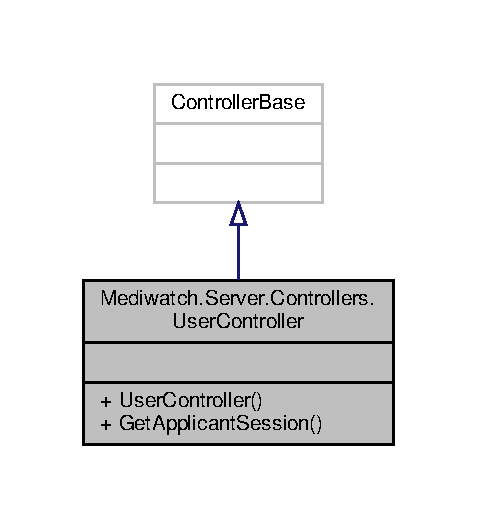
\includegraphics[width=229pt]{class_mediwatch_1_1_server_1_1_controllers_1_1_user_controller__inherit__graph}
\end{center}
\end{figure}


Graphe de collaboration de Mediwatch.\+Server.\+Controllers.\+User\+Controller\+:\nopagebreak
\begin{figure}[H]
\begin{center}
\leavevmode
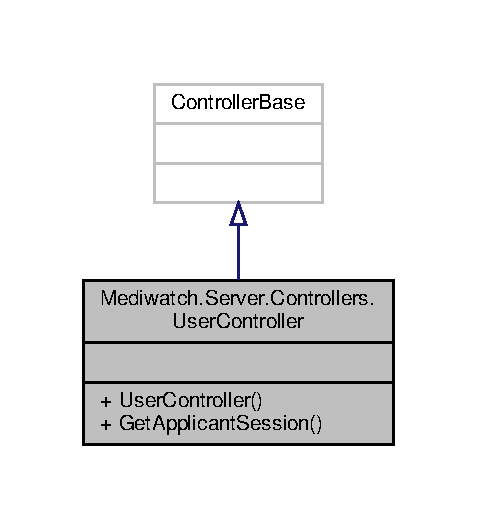
\includegraphics[width=229pt]{class_mediwatch_1_1_server_1_1_controllers_1_1_user_controller__coll__graph}
\end{center}
\end{figure}
\subsection*{Fonctions membres publiques}
\begin{DoxyCompactItemize}
\item 
\mbox{\Hypertarget{class_mediwatch_1_1_server_1_1_controllers_1_1_user_controller_a0824f509c1d9292e4cf6aab3fcf4e659}\label{class_mediwatch_1_1_server_1_1_controllers_1_1_user_controller_a0824f509c1d9292e4cf6aab3fcf4e659}} 
{\bfseries User\+Controller} (User\+Manager$<$ Identity\+User $>$ user\+Manager)
\item 
\mbox{\Hypertarget{class_mediwatch_1_1_server_1_1_controllers_1_1_user_controller_a09c0ab1a896d65d586d34ac6270a2b5c}\label{class_mediwatch_1_1_server_1_1_controllers_1_1_user_controller_a09c0ab1a896d65d586d34ac6270a2b5c}} 
async Task$<$ Action\+Result$<$ I\+Enumerable$<$ Identity\+User $>$ $>$ $>$ {\bfseries Get\+Applicant\+Session} ()
\end{DoxyCompactItemize}


La documentation de cette classe a été générée à partir du fichier suivant \+:\begin{DoxyCompactItemize}
\item 
Server/\+Controllers/User\+Controller.\+cs\end{DoxyCompactItemize}

\hypertarget{class_mediwatch_1_1_server_1_1_controllers_1_1_weather_forecast_controller}{}\doxysection{Référence de la classe Mediwatch.\+Server.\+Controllers.\+Weather\+Forecast\+Controller}
\label{class_mediwatch_1_1_server_1_1_controllers_1_1_weather_forecast_controller}\index{Mediwatch.Server.Controllers.WeatherForecastController@{Mediwatch.Server.Controllers.WeatherForecastController}}


Graphe d\textquotesingle{}héritage de Mediwatch.\+Server.\+Controllers.\+Weather\+Forecast\+Controller\+:
\nopagebreak
\begin{figure}[H]
\begin{center}
\leavevmode
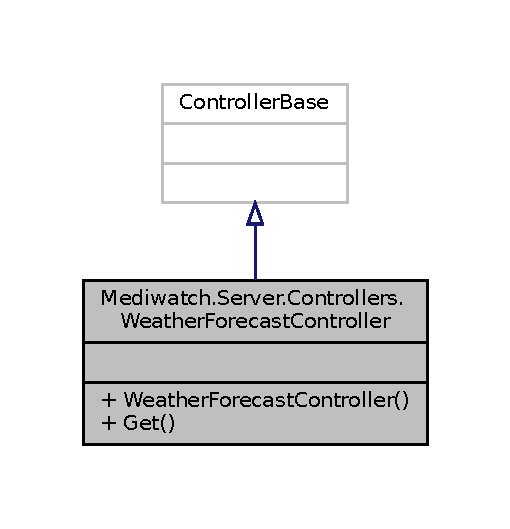
\includegraphics[width=245pt]{class_mediwatch_1_1_server_1_1_controllers_1_1_weather_forecast_controller__inherit__graph}
\end{center}
\end{figure}


Graphe de collaboration de Mediwatch.\+Server.\+Controllers.\+Weather\+Forecast\+Controller\+:
\nopagebreak
\begin{figure}[H]
\begin{center}
\leavevmode
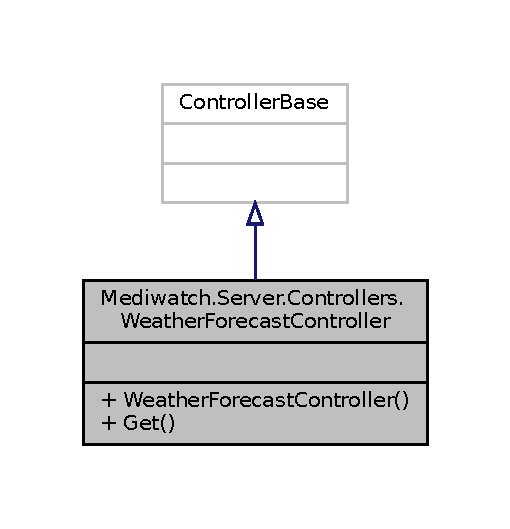
\includegraphics[width=245pt]{class_mediwatch_1_1_server_1_1_controllers_1_1_weather_forecast_controller__coll__graph}
\end{center}
\end{figure}
\doxysubsection*{Fonctions membres publiques}
\begin{DoxyCompactItemize}
\item 
\mbox{\Hypertarget{class_mediwatch_1_1_server_1_1_controllers_1_1_weather_forecast_controller_a8557f93a28d98c9487aa7c812cb61c18}\label{class_mediwatch_1_1_server_1_1_controllers_1_1_weather_forecast_controller_a8557f93a28d98c9487aa7c812cb61c18}} 
{\bfseries Weather\+Forecast\+Controller} (I\+Logger$<$ \mbox{\hyperlink{class_mediwatch_1_1_server_1_1_controllers_1_1_weather_forecast_controller}{Weather\+Forecast\+Controller}} $>$ logger)
\item 
\mbox{\Hypertarget{class_mediwatch_1_1_server_1_1_controllers_1_1_weather_forecast_controller_a43eaa75ecf6f43cba687aeb38a08636f}\label{class_mediwatch_1_1_server_1_1_controllers_1_1_weather_forecast_controller_a43eaa75ecf6f43cba687aeb38a08636f}} 
I\+Enumerable$<$ Weather\+Forecast $>$ {\bfseries Get} ()
\end{DoxyCompactItemize}


La documentation de cette classe a été générée à partir du fichier suivant \+:\begin{DoxyCompactItemize}
\item 
Server/\+Controllers/Weather\+Forecast\+Controller.\+cs\end{DoxyCompactItemize}

%--- End generated contents ---

% Index
\backmatter
\newpage
\phantomsection
\clearemptydoublepage
\addcontentsline{toc}{chapter}{Index}
\printindex

\end{document}
